\documentclass{vldb}
\usepackage{graphicx}
\usepackage{balance}
\newtheorem{example}{Example}
\newtheorem{definition}{Definition}

\begin{document}
\title{Template-based Natural Language Interface for Relational Databases}

\numberofauthors{3}
\author{
\alignauthor Fei Li\\
       \affaddr{Univ. of Michigan, Ann Arbor}\\
       \email{lifei@umich.edu}
\alignauthor
Nikita Bhutani\\
       \affaddr{Univ. of Michigan, Ann Arbor}\\
       \email{nbhutani@umich.edu}
\alignauthor
H. V. Jagadish\\
       \affaddr{Univ. of Michigan, Ann Arbor}\\
       \email{jag@umich.edu}
}

\maketitle

\begin{abstract}
Natural language database interfaces (NLIDBs) are difficult to build because of the ambiguities and implicit assumptions present in natural language.  As humans, we can usually understand a natural language query easily because we have the necessary intuition to help us choose the correct interpretation of the query from among many possible interpretations.  In this paper, our goal is to provide a generic strategy to capture such intuitions and configure them to NLIDBs.  We do this by creating a set of weighted SQL templates to describe likely query logics, in which the weight describes the likelihood of a SQL template to be queried.   When a natural language query is issued, our system maps it to a SQL template based on both its relevance and its weight.  The mapped SQL template is instantiated to a SQL statement, which may include aggregation, nesting, and various types of joins, among many others, and finally is evaluated against an RDBMS.

We have constructed a system, TBNaLIR (Template-Based Natural Language Interface to Relational databases), embodying these ideas. Our experimental assessment demonstrates that TBNaLIR performs very well in practice: a small sized query log is enough to estimate the likelihood of the needed SQL templates, and even naive users are able to get quite complex queries correctly processed using our system.
\end{abstract}

%=====================Introduction=====================================================
\section{Introduction}
\label{sec:introduction}

Querying data in relational databases is often challenging.  SQL is the standard query language for relational databases.  While expressive and powerful, SQL is too difficult for users without technical training.  Even for users with expertise in programming languages, it may still not be easy to use since it requires the users to know the exact schema of the database, the roles of various entities in the query, and the precise join paths to be followed.   As the database user base is shifting towards non-experts, designing user-friendly query interfaces becomes even more important.   

In the real world, people ask questions in natural language.  Not surprisingly, a natural language interface is regarded by many as the ultimate goal for accessing a database, and many natural language interfaces to databases (NLIDBs) have been built towards this goal~\cite{DBLP:journals/nle/AndroutsopoulosRT95,DBLP:conf/iui/PopescuEK03,DBLP:journals/tods/LiYJ07,DBLP:conf/vldb/Minock07,DBLP:journals/pvldb/LiJ14,DBLP:conf/acl/DongL16,DBLP:journals/debu/LuLK16,DBLP:journals/cacm/Liang16,DBLP:journals/tacl/ReddyTCKDSL16}.  NLIDBs have many advantages over other widely accepted query interfaces (keyword-based search, form-based interface and visual query builder).  For example, a typical NLIDB would enable naive users to specify \emph{complex}, \emph{ad-hoc} query intent \emph{without training}.  In contrast, keywords are insufficient to convey complex query intent, form-based interfaces can be used only when queries are predictable and limited to the encoded logic, and visual query builders still require the user to have extensive schema knowledge.

\begin{figure}
  \center
  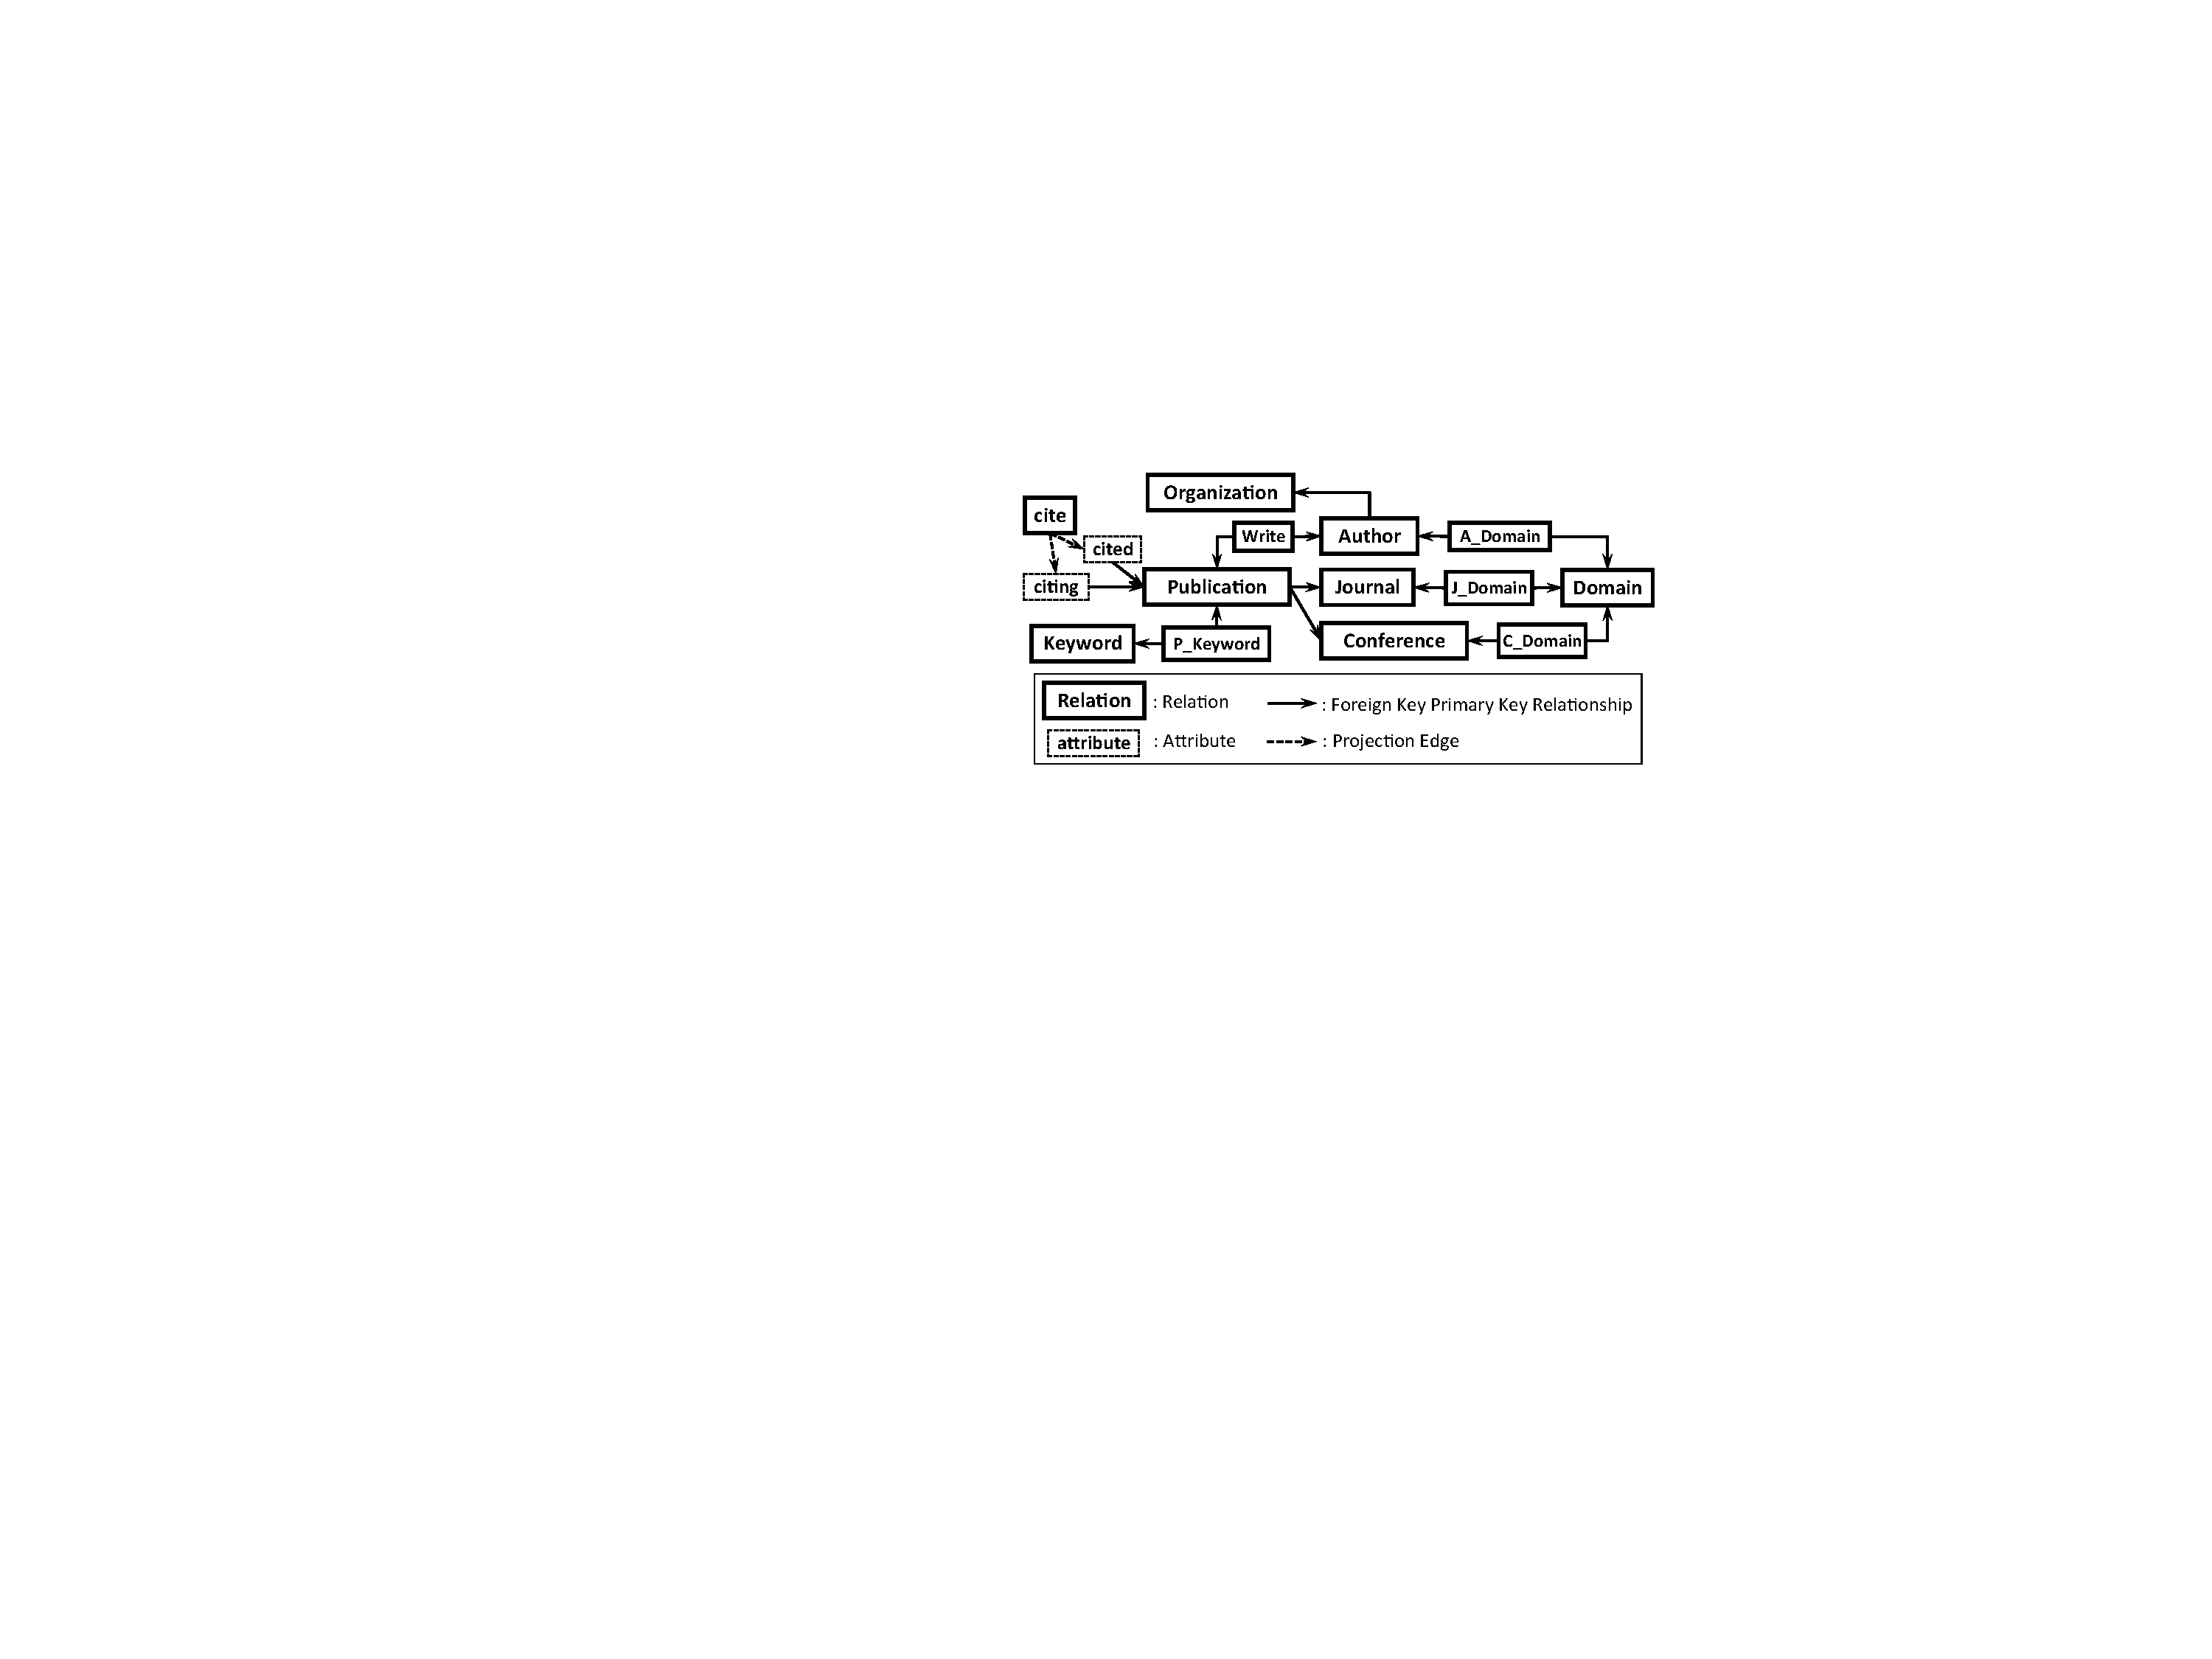
\includegraphics[width=0.95\linewidth]{pic/runningExample.pdf}
  \caption{A Simplified Schema Graph for Microsoft Academic Search}
  \label{fig:runningExample}
\end{figure}

Despite these advantages, NLIDBs have not been adopted widely.  The fundamental problem is that natural language queries are inherently ambiguous.  Even a grammatically correct natural language sentence may contain ambiguities, from both the perspective of natural language processing and the perspective of database schema matching.  Since the number of candidate interpretations grows exponentially with the number of ambiguities, multiple candidate interpretations would be generated and it may be difficult to figure out which one is desired.  
\begin{example}
\label{example:example1}
Consider the query ``show me the citations of ``Constructing an NLIDB..." that are not written by its authors" on the schema graph shown in Figure~\ref{fig:runningExample}.  Many ambiguities exist.  First, the paper has a set of authors and each citation has a set of authors.  It is not clear whether the query requires these two sets to be completely non-overlapping or different in at least one author.  Second, two join paths exist when joining the two papers on the schema graph: (a) $paper_1 \leftarrow citing \leftrightarrow cited \rightarrow paper_2$, in which $paper_2$ is the reference, and (b) $paper_1 \leftarrow cited \leftrightarrow citing \rightarrow paper_2$, in which $paper_2$ is the citation.  It is not easy to figure out which one is desired.  Due to these ambiguities, the NL query can correspond to many SQL statements with semantics that are different, leading to different query results.  
\end{example}

Moreover, naive users often use informal expressions and prefer brevity to logical precision.  
\begin{example}
\label{example:example2}
The query ``authors who have 100 papers" usually means ``authors who have greater than or equal to 100 papers".  The greater than operator in the desired output query is nowhere in the input natural language expression: it has to be deduced from common sense and domain knowledge.
\end{example}

Even though these ambiguities and shortenings are hard for a computer to resolve, we humans can usually tell which interpretation is correct since we can quickly disqualify most other interpretations as unlikely, according to our intuition and common sense.  In this paper, we would like to enable NLIDBs to have this kind of ``intuition" by supporting query logics selectively.  For example, for a bibliographic database, we would expect to support ``which authors have more than 20 papers in SIGMOD?", but not necessarily to support ``which papers have less than 2 authors in Stanford University?", even if these two queries are similar in syntax.  The latter query is perfectly legal, and easily expressed in SQL.  However, based on our domain knowledge and common sense, we can believe that it is an unlikely query.  As humans, when we hear a query like this, our brains go through an error correction process: Did I hear correctly? Could she have meant something else? Is there some other more sensible way I could interpret her question?  We would like to have our system implement the corresponding skepticism.  Similar ideas have previously been suggested, in the context of keyword queries~\cite{DBLP:conf/cidr/NandiJ09}. 

Most natural language query systems generate multiple possible interpretations and use some kind of ranking or scoring mechanism to choose between them.  Typically, this scoring is based only on the relevance of each candidate interpretation of the natural language query.  In contrast, consider search engines, where a keyword query may have many relevant webpages.  In most search systems, the ranking considers both relevance (e.g. using TF-IDF) and the importance of webpages (e.g. estimated using PageRank), as it achieves much higher precision and recall compared to ranking that is based solely on relevance~\cite{DBLP:journals/cn/BrinP98}.  Inspired by this observation, we model the semantic coverage of an NLIDB as a set of weighted {\em SQL templates}, in which the weight describes the likelihood of each template to be queried.  Then, when ranking the candidate interpretations (templates) for a natural language query, we consider the weights of the interpretations as well as the relevance between the query and the interpretations.  

The next immediate question is how to acquire these templates and learn the weights.  In most systems, the query log records the queries issued by actual users.   If a fairly large query log is available, then we can assume that the frequency with which any query logic appears in the query log reflects the probability of a future query being posed with the same logic.   That is, the query log is a representative sample of the distribution of queries.  Based on this idea, we can analyze the query log and define the concept of \emph{popularity} for each SQL template as an estimate of its likelihood to be queried.

Ideally, when we have a large enough SQL query log, it is straightforward to define the popularity for each SQL template based on its frequency.  However, in many real applications, the query log may not be enough to cover all necessary SQL templates.  If the query log is only in natural language, then cost considerations may dictate that only a few queries are manually translated into SQL templates.  Even if all SQL templates are covered, the query distribution, may not reflect the true distribution one would observe with an infinite (theoretical) query log.  DBAs often have a good idea about the domain and typical user interest and are able to distinguish whether a template should or should not be supported based on their expertise.  But it is not realistic to expect DBAs to enumerate all the SQL templates as each template requires time and effort to create.

To address these problems, we provide a strategy to augment the available resources such as query logs and specifications from DBAs.  In our strategy, the existing SQL templates are extended and a PageRank inspired mathematical model is developed for smoothing the popularity of each template.  

Besides mapping to the desired SQL template, the ambiguities at entity level also need to be resolved.  The identification for an entity used in natural language scenarios and that stored in the database are often different.  In a database, keys are defined to uniquely identify entities, while in natural language scenarios, these identifications are often based on attribute values.  However, attribute values stored in the database can be very similar, particularly when they are text strings, and users may not able to specify the exact value for the entity.  We observe that in real world applications, important entities are more likely to be queried (e.g. authors with many papers, papers with many citations, and so forth).  So we formally define the importance for the entities and take it into account for disambiguation at entity level.  

Putting the above ideas together, we propose a framework for NLIDBs comprising two main parts: an offline part, which is responsible for generating weighted SQL templates by analyzing DBA input and the query log, and an online part, which is responsible for translating natural language queries into SQL queries, by mapping and instantiating the SQL templates.  We have constructed such an NLIDB, and we call it TBNaLIR (Template-Based Natural Language Interface to Relational databases).

The intellectual contributions of this paper are as follows: 
\begin{enumerate}
  \item \emph{Weighted SQL Templates.}  We provide a generic method to model the semantic coverage of an NLIDB as a set of weighted SQL templates, in which each SQL template represents a set of SQL queries that differ only in values of constants and the weight of the template describes the likelihood of its being queried.  
   \item \emph{System Architecture.}  We provide a modular architecture for constructing NLIDBs, which consists of an offline part and an online part, in which each component can be designed, and improved, independently.  We develop a working software system called TBNaLIR, which instantiates this architecture. 
  \item \emph{Smoothing Model for Template Popularity.}  We develop a simple probabilistic model,  based on the behavior of a random user, to augment the available resources like query log and DBAs.  Based on this model, we compute popularities for SQL templates, which better reflect the likelihood of each SQL template to be queried, even when the resources are limited.  
  \item \emph{Mapping Strategy.}  We present an effective mapping strategy to map a natural language query to the SQL templates.  The mapping strategy considers not only the relevance between the query and the templates, but also the popularity of the templates.  
\end{enumerate}

The remaining parts of the paper are organized as follows.  In Section~\ref{sec:overview}, we define the SQL template and overview our system architecture.  We extend the semantic coverage of NLIDB in Section~\ref{sec:offline} and computes its popularity in Section~\ref{sec:modelAndPopularity}.  Section~\ref{sec:queryInterpretation} discusses the online processing of a natural language query.  In Section~\ref{sec:experiments}, our system is evaluated experimentally.  We discuss related works in Section~\ref{sec:relatedWork}. In Section~\ref{sec:conclusion}, we draw conclusions and point to future work.

\section{Overview}
\label{sec:overview}
The input to our system is a natural language query whose semantic meaning may involve comparisons, aggregations, various types of joins and nestings, among other things.  The {\em semantic coverage} of our system is defined as a set of weighted SQL templates.  In this paper, each template is weighted by popularity, which describes the likelihood of a template being queried.  Given a natural language query, by mapping it to the correct SQL template, our system translates the natural language query into the desired SQL statement and evaluates it against an RDBMS.  

In this section, we first introduce SQL templates and then describe the system architecture.  

\subsection{SQL Template}
\label{subsec:SQLTemplate}
Two queries are said to have the same {\em query logic} if they have the same SQL structure (SQL keywords, relations, attributes, aggregation functions, operators, nestings), even though constants in the query have different values.  A {\em SQL template} is used to represent such a query logic by replacing the specific values in the SQL statement with slots.  For example, the SQL template of ``papers published after 2007 in VLDB" is shown in Figure~\ref{fig:sampleTemplate}. 

\begin{figure}[h]
\center

\includegraphics[width=1\linewidth]{pic/sampleTemplate.pdf}
\caption{Sample SQL Template.}
\label{fig:sampleTemplate}
\end{figure}

\begin{figure*}
  \center
  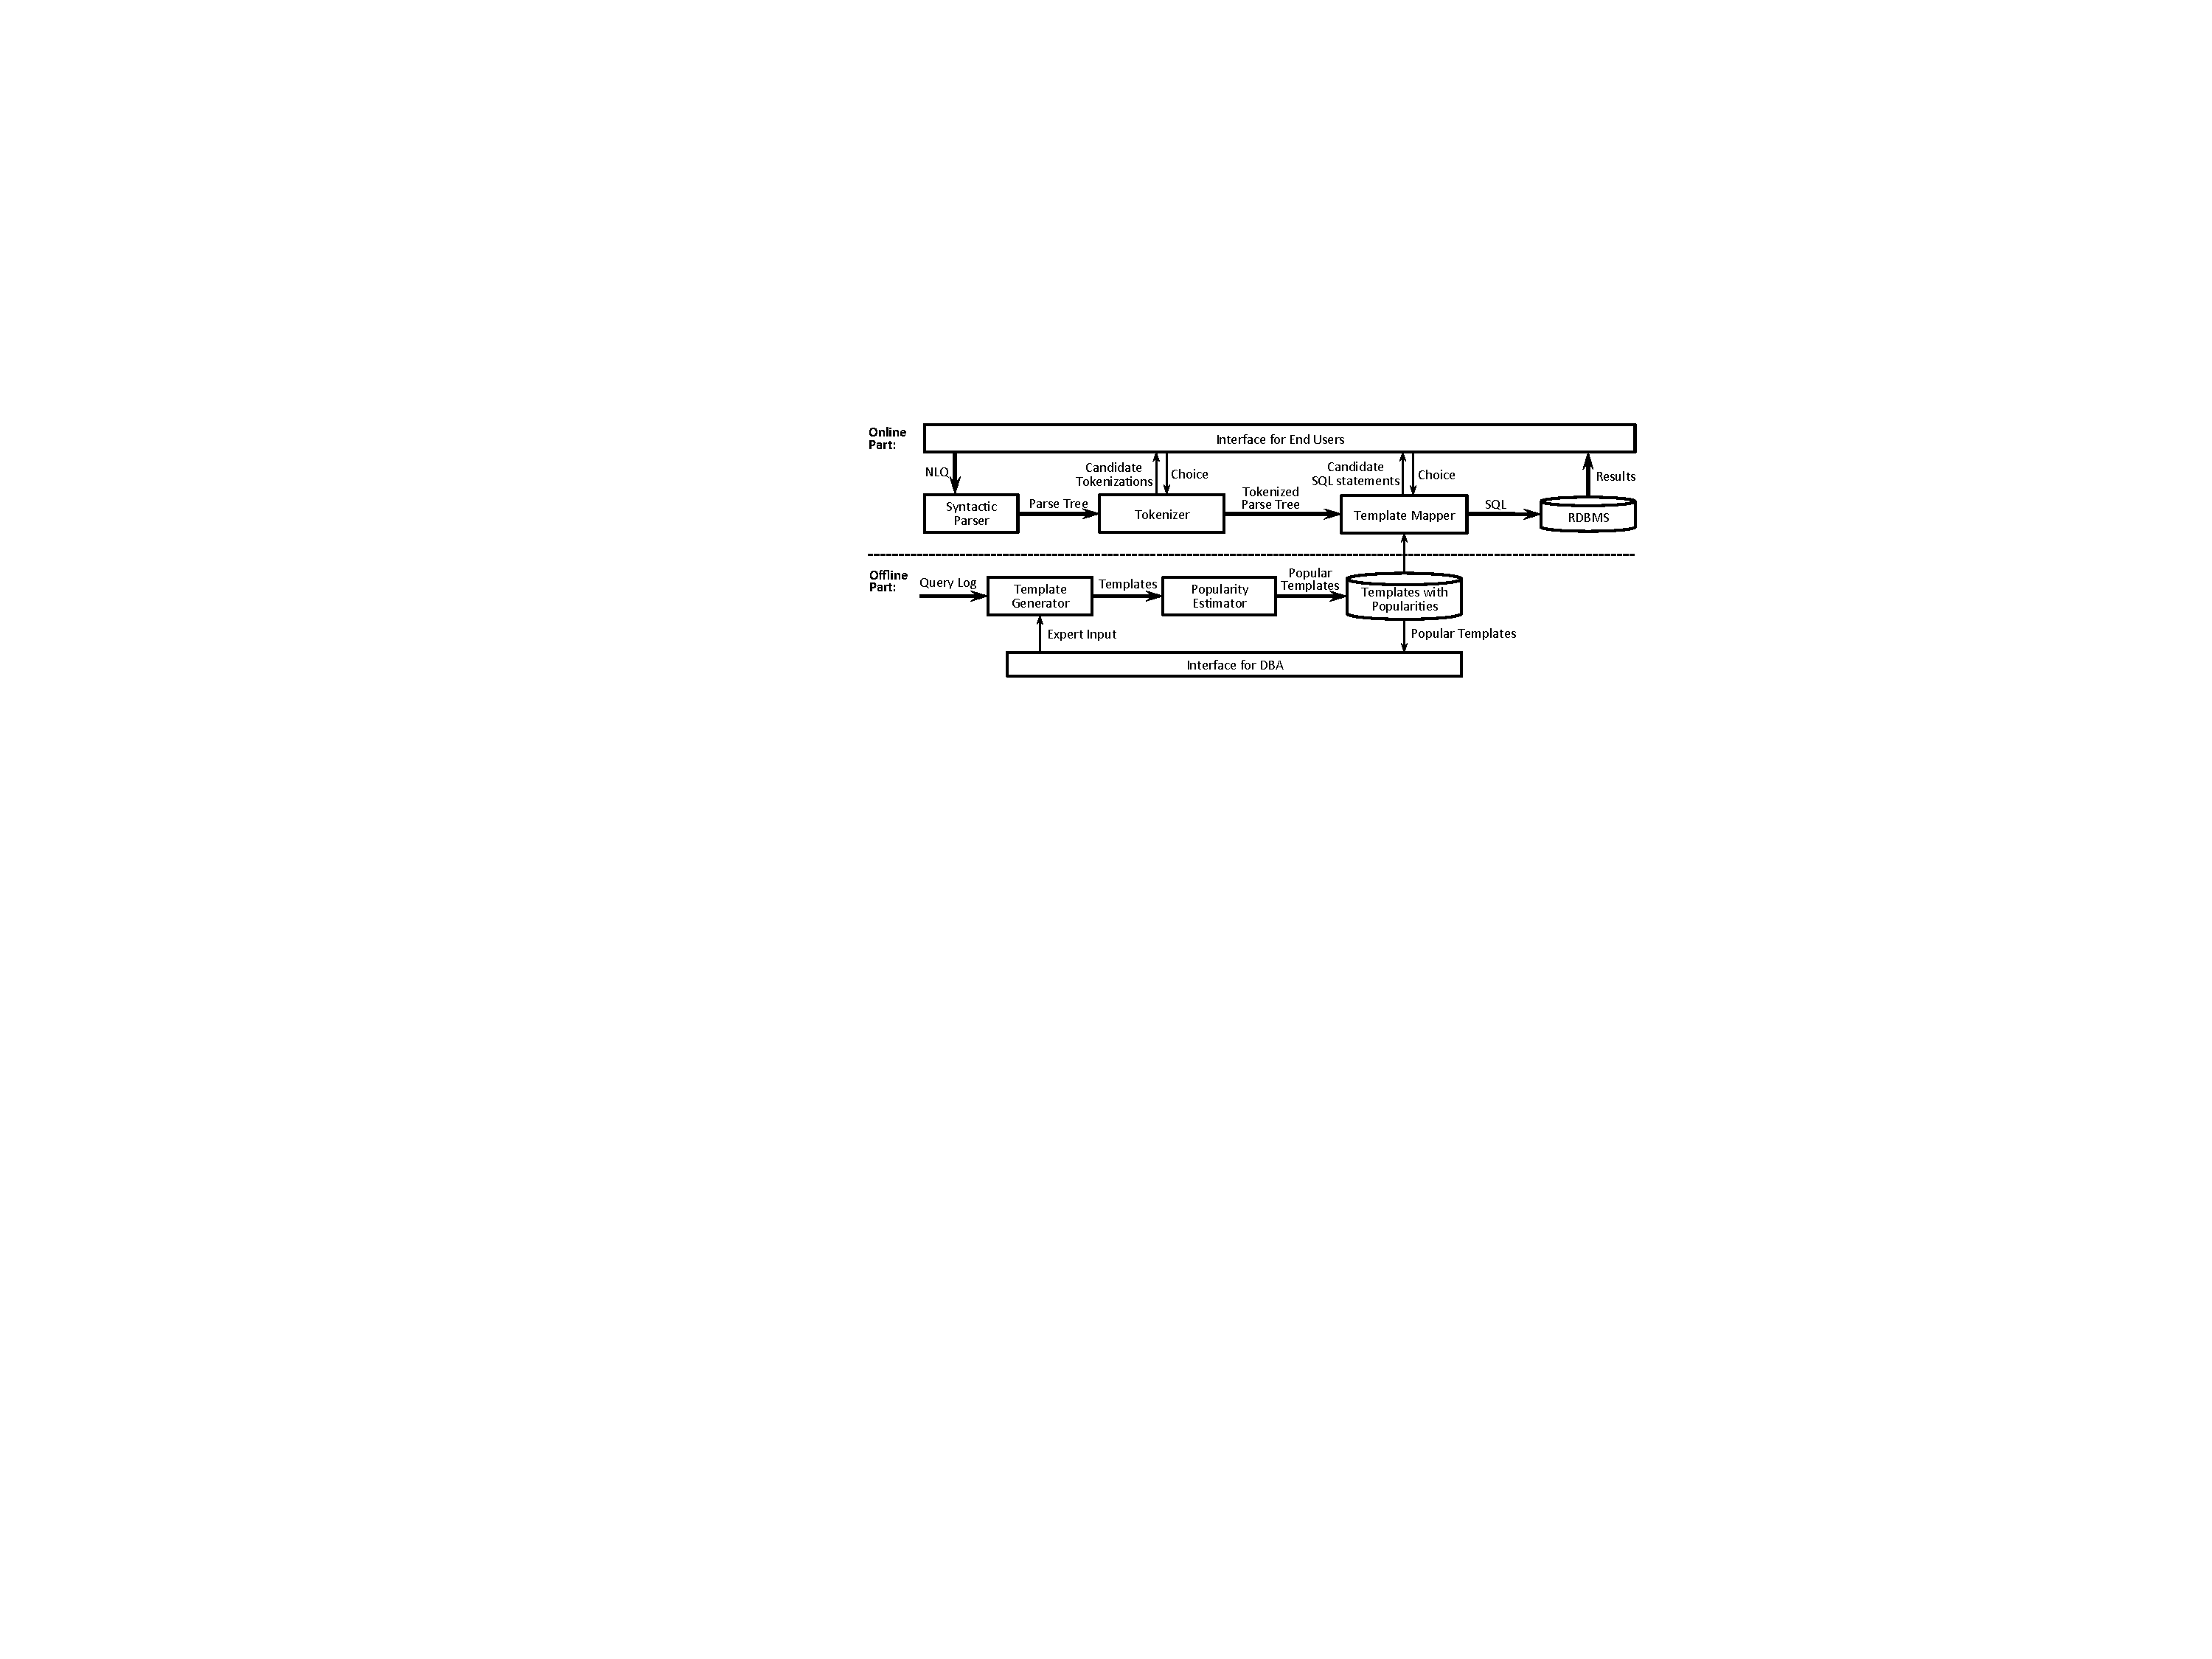
\includegraphics[width=0.9\linewidth]{pic/systemArchitecture.pdf}
  \caption{System Architecture.}
  \label{fig:systemArchitecture}
\end{figure*}

While the values of constants can be ignored in defining templates, it is important to distinguish between related operators.  For example, the SQL templates describing ``authors with $>$ $x$ papers", ``authors with $=$ $x$ papers", and ``authors with $<$ $x$ papers" are considered as three different templates, since they have very different likelihoods of being queried.  The first template is likely to be queried much more frequently than the other two.  As such, it is unfair to define one big template to cover the three and mark all of them as high quality query logics.  Similarly, SQL templates with different operators, quantifiers, aggregation functions, or logic keywords (AND, OR)  should be considered as different SQL templates.  

\subsection{Problem Definition}
The problem we attempt to address is to translate a natural language query (NLQ) to a SQL statement.  In recent works, this problem is often modeled as a semantic parsing problem or machine translation problem, in which the translator is learned from a considerable number of (NLQ, SQL) pairs~\cite{DBLP:conf/acl/DongL16,DBLP:journals/debu/LuLK16,DBLP:journals/cacm/Liang16,DBLP:journals/tacl/ReddyTCKDSL16}.  However, unlike typical semantic parsing or machine translation problems, the underlying schema of different databases often differs, which means the training set for one NLIDB cannot be applied to another NLIDB.  As a result, in real database applications, a good training set is often not available.  That makes the configuration of an NLIDB hard, even if the learning strategy may work in theory.  \cite{DBLP:conf/sigmod/ZhengZLYSZ15} focuses on the generation of training examples, but it still requires a set of natural language queries, which is often not available for relational databases.  

Furthermore, unlike the general problem of semantic parsing or machine translation, an NLIDB has many unique resources for resolving ambiguities, like the underlying schema structure, the query log, the distribution of the data, the configuration from the DBA, and so forth.
The fact that more resources can be taken into account often means higher dimensions of input, which exacerbates the shortage of training examples for a learning-based system.  Instead, we observe that the essence of taking usage of these resources is that they reflect the likelihood of different query logic to be asked.  Therefore, our solution is to capture this information about NLIDB structure and domain in the form of SQL templates.
\begin{example}
Consider Example~\ref{example:example1} where the two ambiguities mentioned would make up four different interpretations, which corresponds to four SQL templates.  By checking the query log (if there is a fairly large one), it is very likely that the SQL template corresponding to the correct interpretation appears much more frequently than the other three.  This information obtained from the query log could serve as a strong evidence for solving these ambiguities.  Similarly, other resources such as the underlying data distribution can also serve as evidences for resolving some ambiguities.  For example, consider the second ambiguity in Example~\ref{example:example1} of generating join paths between two papers.  When examining the data distribution of the underlying database, we could find that the number of references of a paper ranges from 0 to several hundred, while the number of citations of a paper ranges from 0 to tens of thousands.  The distribution of the latter has a much larger entropy, which means a query on that is more informative.  This evidence could also help us to resolve some of the ambiguities.
\end{example}

%\begin{example}
%The ambiguity mentioned in Example 2 can also be solved when a query log is available.  Even in the cases there is no query log, other resources like the data distribution can help to infer the user intent in two steps: (1) in the database, the number of papers by each author iterates most of the numbers from 1 to 1000, which means the distribution is rather ``continuous".  In such kind of distribution, users are more likely to query a range rather than a single point.  (2) In this distribution, most of the numbers are less than 10, which means larger ones are special while small ones are common.  Users are more likely to query special facts (more informative in information theory) rather than common facts.  As such, the system would infer that the user is more likely to mean the query ``authors with more than or equal to 100 papers".
%\end{example}

The {\em semantic coverage} of an NLIDB is the set of all questions that it can support.  It may be possible to state natural language queries outside the semantic coverage, but the system would not be capable of answering these.  We model the semantic coverage of an NLIDB as a set of weighted SQL templates, in which the weights represent the likelihood of each SQL template to be queried.  Given this representation, the problem of understanding an NLQ is naturally modeled as a mapping problem, which tries to map the NLQ to its corresponding SQL template.  The mapping would based on the both the relevance between the NLQ and the SQL template, and the weight of the SQL template.

The system is naturally divided into two parts.  The offline parts obtains the weighted SQL templates from available resources, including user logs and DBA directives.  The goal is to make the SQL templates cover most of the likely NLQs and the weights to faithfully reflect their likelihood to be queried.  The online part maps the input NLQ to the SQL templates.  The goal is to improve the ranking to make the desired interpretation rank higher.

\subsection{System Architecture}
Figure~\ref{fig:systemArchitecture} depicts the architecture of our system. It consists of two main components: an offline part and an online part.  

\subsubsection{Offline Part}
The offline part, which consists of Template Generator and Popularity Estimator, is responsible for generating the weighted SQL templates as the semantic coverage from available resources.  

\paragraph*{Template Generator}
The template generator first transforms each SQL statement in the query log or specified by DBAs into a SQL template.  This set of SQL templates forms the initial semantic coverage.  Given the fact that these resources may be limited or biased, the initial semantic coverage may not be able to cover all (or most of) the likely queries.  To deal with this problem, the template generator extends the initial semantic coverage by generating new SQL templates.  This expanded set of SQL templates serves as a superset of the final semantic coverage of our system.  

\paragraph*{Popularity Estimator}
As will be discussed in detail in Section~\ref{sec:offline}, the SQL templates are not independent of one another.  Templates that share common structures are considered to be relevant to each other.  The Popularity Estimator uses this relevance relationship and a probabilistic model inspired from Pagerank to smooth the weight for each SQL template.  The weight for each SQL template is defined as its popularity, which captures the following intuitions: (1) templates appear frequently in the query log tend to have high popularity, (2) templates relevant to many popular templates tend to be popular, and (3) If a SQL template is specified by an DBA that should (not) be supported, its weight and the weights of its relevant templates should increase (decrease).  Finally, the SQL templates with high popularity are selected to form the semantic coverage of the NLIDB.  

\paragraph*{Interface for DBA}
The interface for DBA helps DBAs to manage the semantic coverage in a semi-automatic manner.  The command of adding a new important SQL template may finally result in adding a series of SQL templates that are missing, while the command of deleting an existing popular template may decrease the weights of many its relevant SQL templates.  It helps the DBAs do the modifications interactively, in which a few iterations would improve the semantic coverage a lot.  

\subsubsection{Online Part}
The online part, which mainly consists of Tokenizer and Template Mapper, is responsible for mapping the natural language query to the correct SQL template and generating the SQL statement.  

\paragraph*{Syntactic Parser}
The first obstacle in translating a natural language query into a SQL query is to understand the natural language query linguistically.  In our system, we use the Stanford Parser~\cite{Marneffe06generatingtyped} to generate a linguistic parse tree from the natural language query.  The linguistic parse trees in our system are dependency parse trees, in which each node is a word/phrase specified by the user while each edge is a linguistic dependency relationship between two words/phrases.  We use dependency parser since it is regarded more stable for relation detection by capturing long-distance dependency~\cite{DBLP:journals/sigmod/NakasholeWS13}.  

\paragraph*{Tokenizer}
In a dependency parse tree, each node is a single word.  The tokenizer identifies the sets of nodes in the linguistic parse tree that can be mapped to database elements (SQL keyword, schema elements and values in the database).  In this process, a set of words may be merged into a phrase, which should be taken as a whole to form a single token.  Given the fact that important database elements are more likely to be queried, the mapping is based on the importance of elements, in addition to the similarity between phrases and the database elements.  

\paragraph*{Template Mapper}
The next step is to understand the relationship between the tokens and interpret the whole query.  In the template mapper, a natural language query is interpreted by finding its corresponding SQL template.  Specifically, our system ranks SQL templates based on both their popularity and their relevance to the input query.  The top SQL templates are instantiated and explained to the user. The one chosen by the user (or the top one by default) is evaluated against the RDBMS.

\paragraph*{Interface for End Users}
To deal with the possibility that  the system possibly misunderstands the user, our system explains to the user how her query is processed.  Specifically, interactive communications are organized in two steps, which verify the intermediate results of the tokenizer and the template mapper, respectively.  For each ambiguity, our system generates a multiple choice selection panel, in which each choice corresponds to an interpretation.  Each time a user changes a choice, our system immediately updates the results in later steps.   

\section{Template Generation}
\label{sec:offline}
We notice that the syntactically valid SQL templates actually form an open set, in which most tepmplates are not semantically meaningful and will almost never be queried by real users.  Our goal is to develop enough SQL templates to cover all reasonable queries while ensuring that there are not too many unnecessary SQL templates.  We develop these templates based on the query log and the specifications from the DBAs using a three-step process as follows: 
\begin{enumerate}  
\item \textbf{Initialization}: Obtain the initial SQL templates that directly appear in the query log or specified by DBAs.  
\item \textbf{Extension}: Extending the initial semantic coverage by generating new SQL templates.  
\item \textbf{Refinement}: Compute the popularity of the SQL templates and choose top ones as the final semantic coverage.\end{enumerate}
In this section, we discuss the first two steps.  The refinement step will be described in the next section.

The initialization step is quite straightforward, according to the definition of SQL template.  Given the fact that the queries in the query log may be limited or biased, not only can we be off on the frequencies of SQL templates that occur, it is also possible that we entirely miss templates that do occur in practice but happened not to be present in our small sample. This danger is exacerbated by our need to distinguish between operators and query structures at fine granularity, which increases the number of SQL templates we need to support. Similarly, it is usually easy for an expert DBA to fast design some likely query templates, but it is very hard to be complete and make sure not to miss any likely query templates.  So, in the extension step, the initial semantic coverage, whether obtained from query log or DBA,  is extended by adding new SQL templates.  

We define an {\em SPJA template} to be a SQL template that uses only selections, projections, FKPK (foreign-key-primary-key)  joins and aggregations (including Group By and Having clauses).  We first describe how SPJA templates are generated in the next several paragraphs, and then extend complex templates later in this section.
\begin{example}
Given the simplified schema shown in Figure~\ref{fig:runningExample}, the SQL template for the query in Example~\ref{example:example1} is a complex (non-SPJA) template, which involves subquery with a NOT IN clause.  The query in Example~\ref{example:example2} can be expressed by an SPJA template.  
\end{example}

We start from the generation of SPJA templates.  A similar problem arises in schema-based keyword search~\cite{DBLP:conf/vldb/HristidisP02,DBLP:conf/sigmod/MarkowetzYP07,DBLP:conf/icde/FanLZ11,Li:2014:SS:2588555.2588571}.  However, we cannot simply adopt their method since too many SQL templates would be generated, in which most of them are semantically meaningless, especially when aggregations are considered.  
\begin{example}
\label{example:distribution}
Given a simple join path, paper - citing - cited - paper, many SQL templates can be generated.  Here we choose two of them as examples, which correpsond to ``papers with more than 1000 citations" and ``papers with more than 1000 references", respectively.  As humans with experiences in querying bibliographic databases, we could easily tell that the first one is much more likely to be queried than the second one.  But how to provide the system with such intuition? 
\end{example}

Here we take into account the underlying data distribution to distinguish semantically meaningful SQL templates from others.  In Example~\ref{example:distribution}, we observe that the number of citations for each paper ranges from zero to tens of thousands, while the number of references in each paper ranges from zero to several hundreds at most.  Obviously, the former distribution is much more dispersed than the latter.   In information theory, the entropy of the former would be higher, which means a query on that is more informative.  We adopt the concept of entropy from information theory to estimate whether an SPJA template is semantically meaningful.
\begin{definition}[Fanout Set]
Let $R$ be all the schema elements returned, $J$ be the FKPK join network at schema level, $\{r_{i}\}$ be the combination set of the tuples of $R$, $j_r$ be the join networks corresponding to $J$ at tuple level that contains the tuple combination $r$.  The fanout set of the SQL template is defined as $M = \{|j_r|\ |\ r\in\{r_i\}\}$.  
\end{definition}

Given the fanout set $M$, let $\{m\}$ be its distinct values and $f_m$ be the relative frequency of $m$.  The entropy of $M$ is computed as follows: 
\begin{equation}
E(M) = -\sum_{m \in M}  f_m \cdot \log f_m
\end{equation}
The entropy is then normalized to a number between 0 and 1, and a threshold is used to filter out the templates with low fanout entropies.  

Given this concept, the system is automatically configured with a rough intuition of which SQL templates are more likely to be queried.  For example, when generating the SQL templates containing two authors, the system is able to figure out that ``the authors who coauthored with Bob" is more semantically meaningful than ``the authors who are in the same organization as Bob", while ``the authors who are in the same research domain with Bob" is essentially meaningless.

For complex templates, it is difficult to construct the special structures (non-FKPK joins, set operations, nestings) from scratch.  Instead, we generate new complex templates only by modifying the complex templates that directly appear in the query log.  Specifically, we modify the SPJ parts of complex templates by adding/deleting constraints.  Consider the SQL template mentioned in Example~\ref{example:example1} again.  Given the SQL template of ``show me the citations of `Constructing an NLIDB...' that are not written by its authors", we are able to generate the SQL templates like ``show me the citations of `Constructing an NLIDB...' that are \emph{published in VLDB} and are not written by its authors" by modifying its SPJ parts.  

Additionally, we also allow DBA to specify templates that should NOT occur.  This expert input can occasionally be valuable: for example, if the small query log has some idiosyncratic queries that are better ignored, or to guide our template set extension method described above by limiting some templates.  These templates are simply recorded with a negative appearance at this stage.  The weight will be smoothed in the next stage, described in the next section.

\section{Popularity}
\label{sec:modelAndPopularity}
Ideally we would like to have a sufficiently long query log that records the querying behavior of actual users.  In this case, we can assume that the log includes all the necessary SQL templates with frequency proportional to the real distribution, and the appearance frequency of a SQL template can be used directly to reflect its chances to be queried again.  

In practice, the resources available are often limited, and may be artificially derived as discussed above.  In this case, we must worry about the query log not being a good representative sample of the entire distribution.  In this section, we provide strategies to smooth the weights for the SQL templates, which makes them reflect their likelihood of being queried, even in the cases when the resources are limited. 

\subsection{Template Relevance}
\label{subsec:model}

A central observation on which we base our smoothing model is that the SQL templates are not independent of one another.  As such, if a template is considered important and has a high weight (e.g. appears frequently in the query log), other templates it  includes, or that include it, should also be given some credit.  We call such other templates {\em relevant} to the target template.
\begin{example}
Consider the SQL templates show in Figure~\ref{fig:relevantQueries}.  Intuitively, if $T_1$ appears frequently in the query log, $T_2$ should also be assigned some weight.  Similarly, if $T_3$ is specified by an DBA as one that should not be supported, the weight of $T_4$ should also be reduced.  
\begin{figure}[h]
  \center
  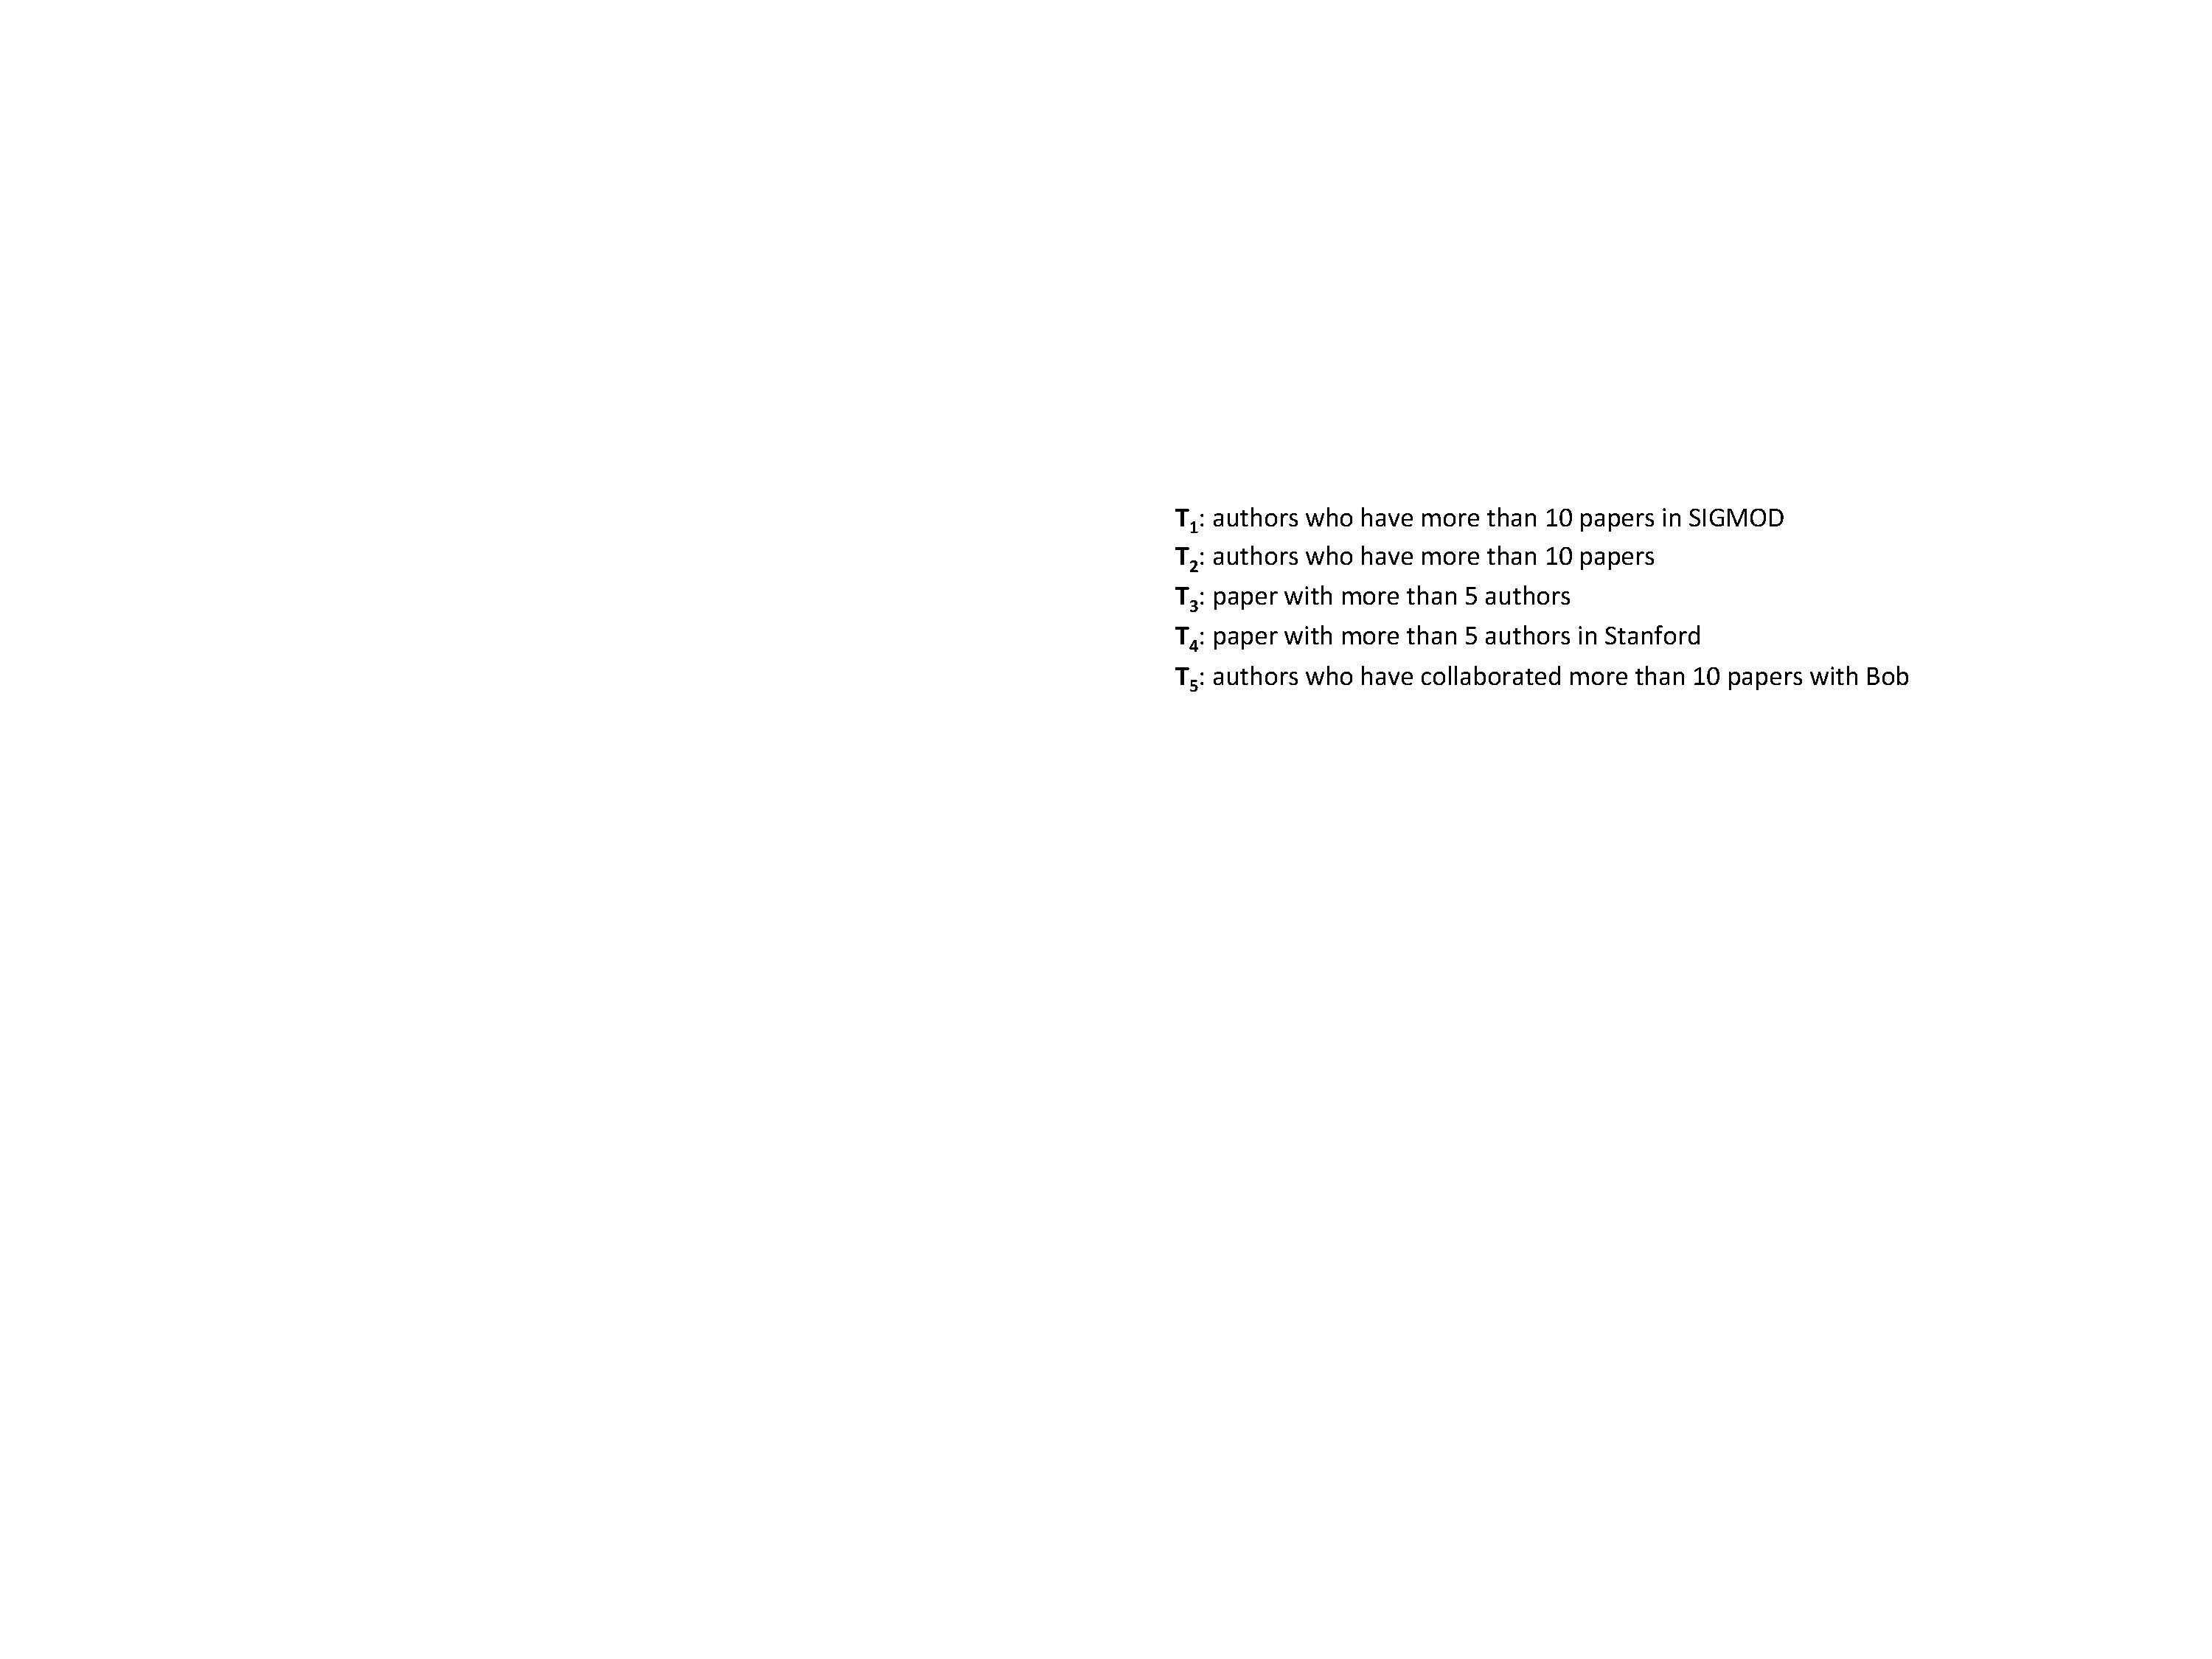
\includegraphics[width=0.9\linewidth]{pic/SPJQuery2.pdf}
  \caption{Pairs of Relevant Queries.}
  \label{fig:relevantQueries}
\end{figure}
\end{example}

To capture this observation, two intuitions need to be quantified: (a) how to evaluate the relevance between two templates and (b) how to smooth the weights by transferring them from one template to its relevant templates.  

In our system, two SQL templates are considered relevant only when the graph representation of one template contains/is contained by the other\footnote{Theoretically, the subgraph isomorphism problem is NP-complete~\cite{DBLP:conf/stoc/Cook71}, with running time that is exponential in the number of the graph nodes with the same label.  In the graphs representing SQL templates, the number of such nodes is typically very small and the efficiency is not a problem. }.  Let $T_1$ and $T_2$ be two SQL templates.  In the cases when $T_1$ contains $T_2$, we define the relevance between them as $\mathit{(\frac{1}{2})^{(\frac{|T1|}{|T2|})}}$, in which $|T|$ is the size (total number of nodes and edges) of template $T$.  This definition is based on the observation that the larger subgraph $T_2$ is of $T_1$, the more relevant they should be.  

This is a rather rigid definition for relevance since only containing/contained relationship is taken into account.  
Indeed, the definition of the relevance between two templates is somewhat subjective, and the specific definition is not material for the rest of our framework.  So a different choice of relevance function can easily be substituted.  However, we point out that similarity through substitution is a bad idea, since that is precisely the type of difference we are trying to tease out, as indicated by the many examples we presented above.  Inclusion, on the other hand, is a much stronger relationship.

As will be discussed in detail in the next section, we put all the SQL templates into a graph, in which two templates are connected by an edge if they are relevant to each other.  A strategy inspired from PageRank is used to smooth the weights of SQL templates.  Using this strategy, the weight of a SQL template can be transferred to another SQL template indirectly, even if they are not directly relevant.
\begin{example}
Consider the SQL templates show in Figure~\ref{fig:relevantQueries}.  $T_1$ is relevant to $T_2$ since the graph representation of $T_1$ contains $T_2$.  Similarly, $T_5$ is relevant to $T_2$.  If $T_1$ appears frequently in the query log, some of its weight can be transferred to $T_5$ through $T_2$.   
\end{example}

\subsection{Popularity of SQL Templates}
\label{subsec:popularity}

In this subsection, we smooth the weight of templates based on following three intuitions:
\begin{enumerate}
  \item A SQL template that appears frequently in the query log should be assigned a high weight.
  \item A SQL template that shows high relevance with many important (high weight) SQL templates should also be assigned a high weight.
  \item If a SQL template is specified by an DBA that should (not) be supported, its weight and the weights of its relevant templates should increase (decrease).
\end{enumerate}

To capture the first two intuitions, we develop a random user query model inspired by PageRank, in which we pretend that after the user composes a SQL query, she is likely to randomly compose a series of follow up queries, each of which is related to the last query.  Of course, we do not expect that real users will actually issue queries in this fashion. In fact, the order in which queries are issued is not of relevance for our purposes.  Rather, what we want to do is to add queries to the limited query log that are relevant to the queries already in the log.  This random follow up query model accomplishes this addition in a principled way.

Here, based on the relevance between SQL templates, we put all the SQL templates into one \emph{Relevance Graph}.  
\begin{definition}[Relevance Graph]
The relevance gr-aph $G(V, E)$ is an undirected graph, in which each node $T_i$ in V is a SQL template.  There is an edge $(T_i, T_j)$ in $E$, if $T_i$ and $T_j$ are related.  A weight $w(T_i, T_j)$ is set for each edge $(T_i, T_j)$ to reflect the relevance between $T_i$ and $T_j$. 
\end{definition}

In the random querying model, we assume there is a ``random user" who compose her first SQL query by randomly choosing one SQL query in the query log.  Then she keeps on composing a series of SQL queries, in which each SQL query is ``related" to the last query she composed.  Eventually, she gets bored and starts on another SQL query in the query log and compose another series of SQL queries.  In this process, the probability that the random user submits the queries in a SQL template is defined as the popularity of that SQL template. 

Suppose that after the random user composes a query in template $T_i$, the user has the probability of $c$ to compose a follow up query and has the probability of $1-c$ to get bored and start to choose a new SQL query in the query log.  If she composes a follow up query, the likelihood of a SQL template $T_j$ to be queried is proportional to the relevance between $T_i$ and $T_j$.  On the other hand, if she gets bored and choose another query in the query log, the likelihood of a SQL template $T_j$ to be queried is proportional to its appearance frequency in the query log.  

In formal notation, let $G = (V, E)$ be the relevance graph and $L$ be the query log, in which a SQL template $T$ appears $l(T)$ times.  $l(T)$ is 0 if $T$ never appears in the query log.  Let $T_i$ and $T_j$ be two SQL templates and $w(T_i, T_j)$ be the relevance between them in $G$.  $w(T_i, T_j)$ is 0 if $T_i$ is not related to $T_j$.  The probability that the user will query $T_j$ after querying $T_i$ is: 
\begin{displaymath}
P(T_j|T_i) = c\frac{|w(T_i, T_j)|}{|\sum_{T_k \in V}w(T_i, T_k)|} + (1-c)\frac{l(T_j)}{|L|}
\end{displaymath}

Given the probability a SQL template $T_j$ to be queried after the SQL template $T_i$, we define the template graph to compute the popularity for each SQL template.  
\begin{definition}[Template Graph]
The template graph $G_T(V, E)$ is a directed graph in which each node $T_i$ in $V$ is a SQL template.  There is an edge $(T_i, T_j)$ in $E$, if $T_i$ and $T_j$ are relevant or $T_j$ appears in the query log.  Specifically, each edge $(T_i, T_j)$ is weighted by $P(T_j|T_i)$.  
\end{definition}

Given the template graph, the computation of the popularity is quite straightforward, and very similar to the computation of PageRank for web pages.  Let $Popularity$ be the vector of the popularities for each SQL template in the expanded semantic coverage.  $Popularity$ is initialized according to the appearance frequency of each SQL template in the query log.  Let $G_T(V, E)$ be the template graph, represented by an adjacency matrix.  By multiplying $Popularity$ with $G_T(V, E)$ for a few rounds until its value converges, the popularity for each SQL template can be obtained.  We then normalize each entry in $Popularity$ into a number between 0 and 1 by first adding it to 1, then taking its binary logarithm, and finally dividing it by the maximum value in the vector.  

When taking the specifications from the DBAs into account, $l(T_j)$ is modified accordingly.  When the DBA specify that $T_j$ should (not) be in the semantic coverage, we modify $l(T_j)$ by adding (subtracting) a big number.  As such, when running the PageRank algorithm, a positive $l(T_j)$ could help $T_j$ to absorb these weights from all the templates in the graph and distribute the weights to $T_j$'s relevant templates.  In a similar manner, a negative $l(T_j)$ could absorb weights from $T_j$'s relevant templates and distribute these weights to all the templates in the graph.  

\section{Online Query Interpretation}
\label{sec:queryInterpretation}

Given an online natural language query represented by a dependency parse tree, we first interpret each of its words and phrases by mapping them to the database elements (SQL keywords, schema elements and database values).  Then, the whole query is interpreted by finding its corresponding SQL templates from among those generated in the offline part.  

\subsection{Element Mapping and Tokenization}
\label{subsec:tokenization}

We first identify the parse tree nodes (words/phrases) that can be mapped to database elements.  Such nodes can be further divided into different types as shown in Figure~\ref{fig:nodeType}, according to the type of database elements they mapped to.  The identification of select node, operator node, function node, quantifier node and logic node is independent of the database being queried.  Following~\cite{DBLP:journals/tods/LiYJ07,DBLP:journals/pvldb/LiJ14}, we enumerate sets of phrases as the database independent lexicon to identify these five types of nodes. 

\begin{figure}[h]
  \center
  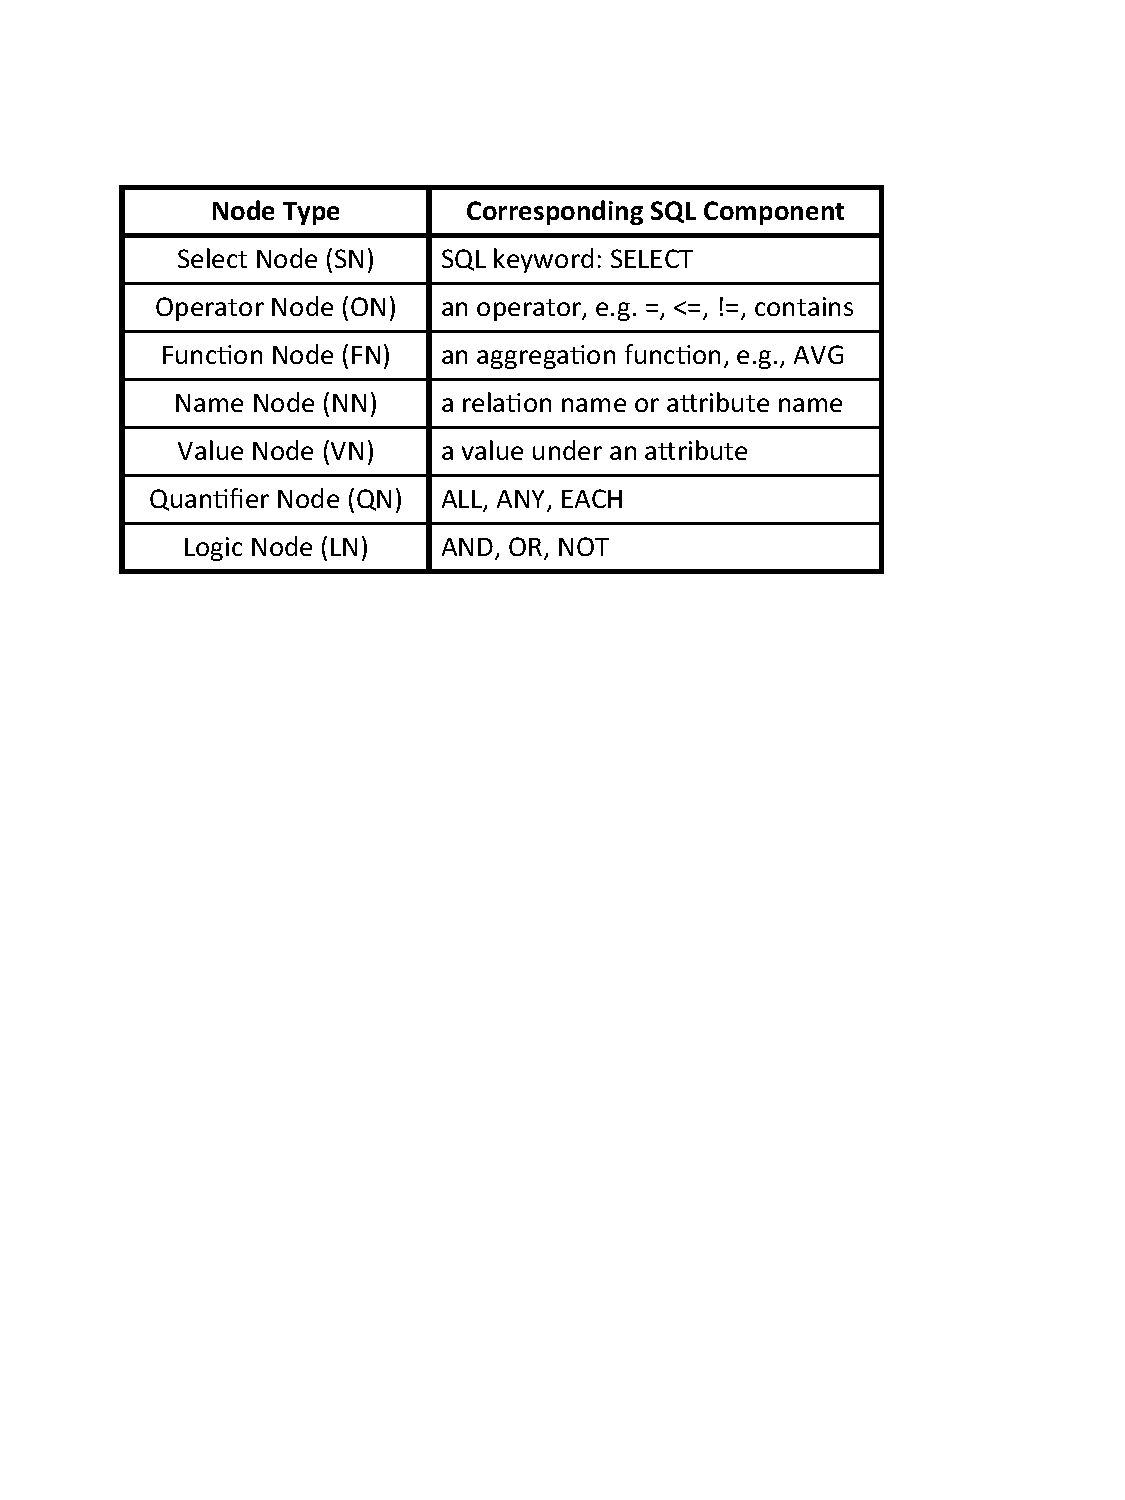
\includegraphics[width=0.8\linewidth]{pic/nodeType.pdf}
  \caption{Different Types of Nodes.}
  \label{fig:nodeType}
\end{figure}

In contrast, name nodes and value nodes correspond to the schema elements and tuples in the underlying database, respectively.  Often, the words/phrases specified by the user are not exactly the same as the ones stored in the database.  In previous literature, the mapping is typically based only on the similarity between the words/phrases, with possible thesaurus expansion,  and the schema elements/tuples in the database.  However, one should expect that important schema elements/tuples are more likely to be queried.  For example, an author name specified by the user may have multiple mappings in a bibliography database.  The important ones (with many papers with many citations) are more likely to be the one in the user's mind.  In this paper, we formally capture this intuition and define the importance for the schema elements and tuples in the database.  

\begin{definition}[Tuple Importance]
Represent the given database as a directed data graph, in which each node is a tuple in the database and each edge is a foreign-key-primary-key (FKPK) relationship between two tuples\footnote{To avoid the situation that the importance gets "trapped" in tuples with no outgoing links, we add both a PK-FK edge and an FK-PK edge in the data graph to represent an FKPK relationship in the database.}.   The unnormalized importance of each tuple is defined as $log_{2} (pagerank)$, in which pagerank is its pagerank~\cite{Page99thepagerank}.  
\end{definition}

\begin{definition}[Schema Element Importance]
Let $S$ be the semantic coverage generated in the offline part of our system.  The unnormalized importance of each schema element is defined as $(\sum_{T} Popularity(T))$, in which $T$ iterates over all the SQL templates in $S$ that contain the schema element.  
\end{definition}

The importance of each tuple (resp. schema element) is then normalized to a number between 0 and 1 by dividing it by the maximum  importance of any tuple (resp. schema element) in the database.

In this paper, we map the nodes to the schema elements and tuples based on both similarity and importance.  Let $n$ be a word or a phrase and $v$ be a schema element or a tuple.  The goodness of the mapping between them is scored as follows: 
\begin{displaymath}
Score(n, v) = Similarity(n, v) + \mathit{Importance(v)}
\end{displaymath}

Specifically, the similarity between a node and a schema element is defined as the max of their semantic similarity (WUP similarity~\cite{DBLP:conf/acl/WuP94} based on wordnet) and their spelling similarity (square root of the coefficient of their q-gram sets~\cite{DBLP:journals/tods/XiaoWLYW11}).  The similarity between a node and a tuple considers only their spelling similarity, for efficiency reasons.  

For each node, the best mapping is set as the default interpretation for the node, but the user is shown the top $k$ mappings as alternatives to choose from.   Given the vocabulary restriction of the system, some parse tree nodes may fail in mapping to any type of tokens.  In such a case, a warning is generated, showing the user a list of nodes that do not directly contribute in interpreting the query.  Our system deletes each such node from the parse tree and moves all its children to its parent.  

\subsection{Template Mapping}
\label{subsec:mapping}

%After the tokenization, 
%(possibly with some feedback from the users), IT HURTS YOU TO TALK REPEATEDLY ABOUT FEEDBACK
%we assume that each node in the dependency parse tree is perfectly understood.  
In this section, we interpret the whole query by mapping it to the SQL templates generated in the offline part.  Given a natural language query $\mathit{NLQ}$, represented by a tokenized parse tree, its mapping score to a SQL template $T$ is define as: 
\begin{displaymath}
Score(\mathit{NLQ}, T) = Relevance(\mathit{NLQ}, T) + Popularity(T)
\end{displaymath}

Specifically, $Popularity(T)$ is the popularity defined in Section~\ref{subsec:popularity}.  $Relevance(\mathit{NLQ}, T)$ is the relevance between $\mathit{NLQ}$ and $T$.  Given the fact that $\mathit{NLQ}$ is represented by a tokenized parse tree, in which trivial nodes have been deleted after the tokenization, most of the information specified in $\mathit{NLQ}$ should be contained by $T$, if it is relevant to $\mathit{NLQ}$.  Reciprocally, one would think most of the information in $T$ should also be contained in $\mathit{NLQ}$.  However, natural language queries tend to be brief and often leave out things that ``can be understood".  Furthermore, natural language queries typically do not include schema-specific constructs such as FK-PK join paths, which are often by-products of normalization.  So, in the reciprocal direction, we expect that most of the {\em major} information in $T$ should also be contained in $\mathit{NLQ}$, according to a definition of {\em major} that we provide in the next paragraph.  Putting these ideas together, $\mathit{NLQ}$ is considered relevant to $T$ if (a) the information in $\mathit{NLQ}$ is contained by $T$, and (b) the major information in $T$ is specified in $\mathit{NLQ}$.  In particular, we define their relevance as follows: 
\begin{displaymath}
\mathit{\frac{|Info(NLQ) \cap Info(T)|}{|Info(NLQ)|} * \frac{|MInfo(NLQ) \cap MInfo(T)|}{|MInfo(T)|}}
\end{displaymath}

We define $\mathit{Info(NLQ)}$ as the set of ($parent$, $child$) relationship in $\mathit{NLQ}$.  $Info(T)$ as the set of ($node_i$, $node_j$) in $T$, in which $node_i$, $node_j$ are \emph{referred nodes} in $\mathit{NLQ}$ that are \emph{directed related}.  In this paper, referred nodes are the nodes in $T$ that are referred to by the query $\mathit{NLQ}$.  Directly related means there is a path between $node_i$ and $node_j$, which is not interrupted by other referred nodes.  $\mathit{MInfo(NLQ)}$ is the set of nodes in $\mathit{NLQ}$, while $\mathit{MInfo(T)}$ is all the \emph{major nodes} in the SQL template $T$.  The major nodes are the nodes whose information is important and unlikely to be omitted by the user.  For example, $\mathit{MAX}$ is a major node, which is not likely to be omitted by the user, while $\mathit{COUNT}$ is not a major node, since it is often implicit in the user's query.  We enumerate the set of major nodes, which serves as the knowledge base that can be used independent of domains.  

\section{Experiments}
\label{sec:experiments}

In our system, the quality of the semantic coverage, which is automatically generated in the offline part, directly affects the behavior of the online part.  As such, we first evaluate the offline part separately and then show the benefits it brings for the online part.  

\textbf{Dataset.}
The dataset we use is Microsoft Academic Search (MAS), whose simplified schema graph is shown in Figure~\ref{fig:runningExample}.  Some summary statistics of its major relations are shown in Figure~\ref{fig:statistics}.  

\begin{figure}
  \center
  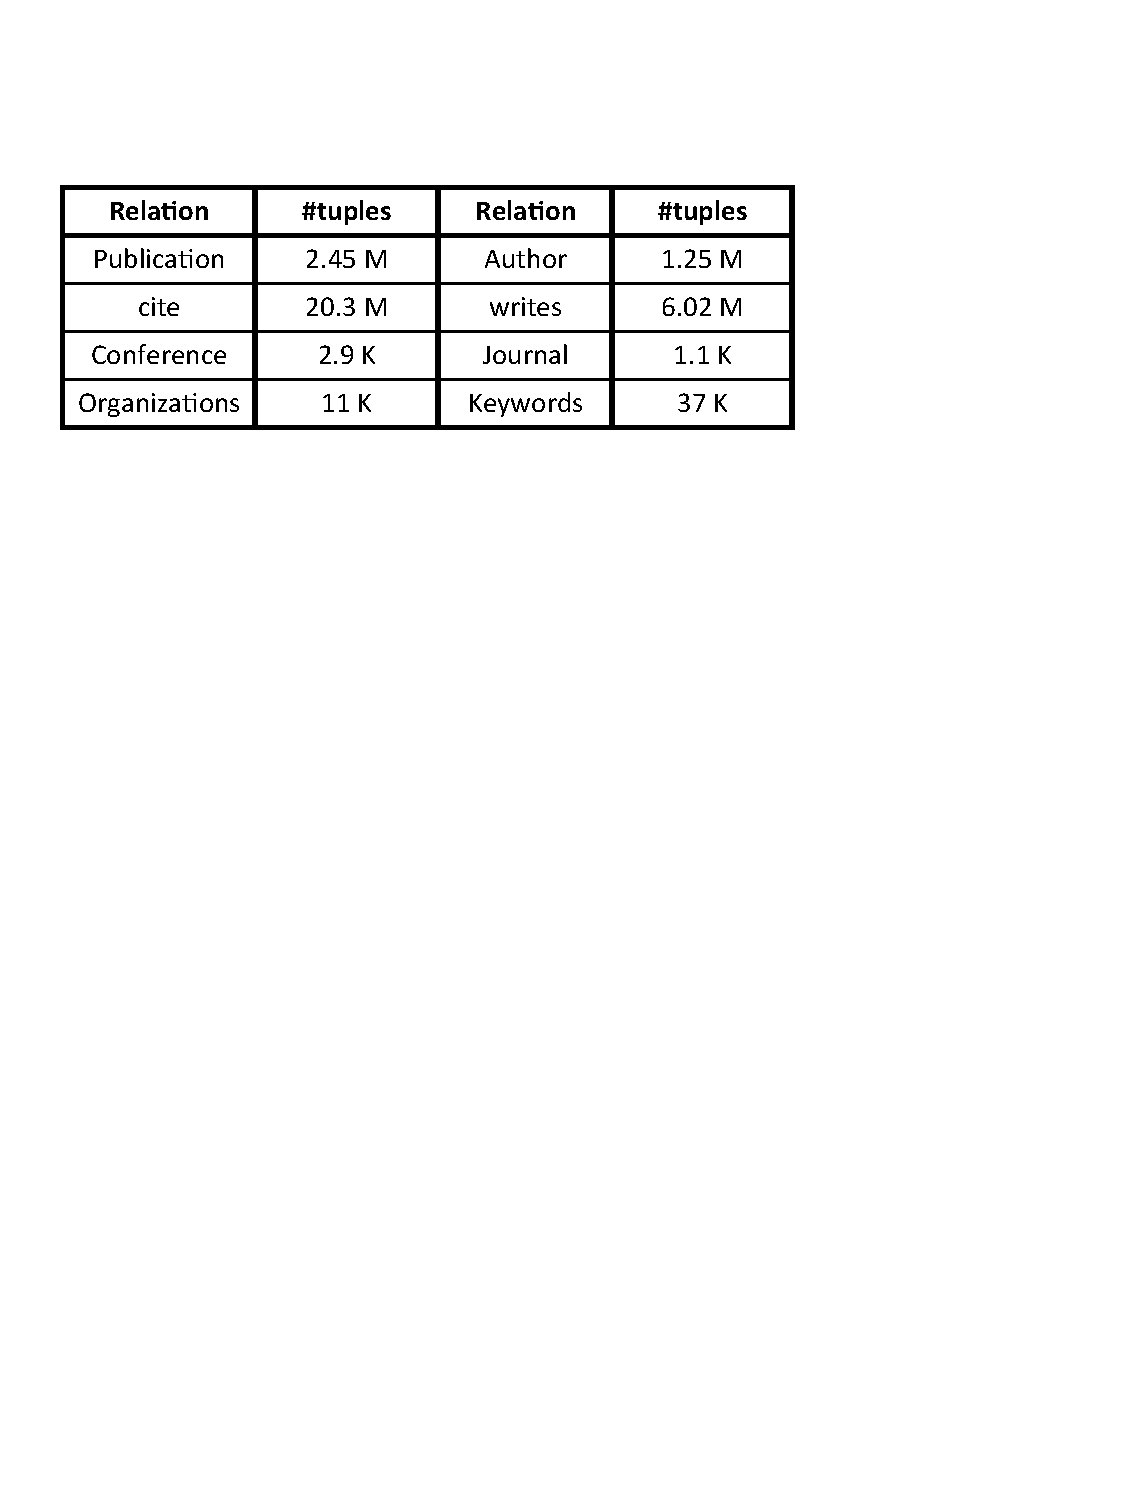
\includegraphics[width=0.8\linewidth]{pic/statistics.pdf}
  \caption{Summary Statistics for MAS Dataset.}
  \label{fig:statistics}
\end{figure}

\subsection{Offline Part}
\label{subsec:experiments_offline}
The goal of the offline part is to generate a high quality semantic coverage, in which most of the necessary query logics are covered, while including as few additional (unnecessary) query logics as possible.  Adopting standard terminology from information retrieval, we would like to create a set of query templates that has very high recall (coverage is good) and acceptable precision (not too many unnecessary templates in the set).  Since, practically speaking, our direct concern is with the size of the set created, we report this size directly, rather than the precision that it is roughly proportional to.  

\textbf{Test Set (Gold Standard).}
To evaluate the recall of a semantic coverage, we need a gold standard.  The old version interface of MAS dataset was a carefully designed faceted interface.  By clicking through the site, a user is able to get answers to many quite complex queries.  We enumerated all query logics that are directly supported by the MAS website and obtained a set of 196 SQL templates.  We noticed that the semantic coverage of the MAS website was constrained by the overall design of the interface. As a result, some likely query logics are not supported because they would require a redesign of the interface and impact the overall visual effect. Also, it is possible that some unnecessary query logics are supported just because they are more compatible with interface.  This is a common limitation of forms-based interfaces, faceted interfaces and WIMP (windows, icons, menus and pointers) interfaces.  To address these shortcomings, we asked five domain experts, who often do academic searches and have a good sense of which questions would be frequently asked over a bibliographic database, to modify this set of query logics, deleting unnecessary ones and adding new ones as needed.  In this process, we accepted a modification only when it had the agreement of all five experts. The final test set $Q_{gold}$ we obtained is composed of 160 SQL templates, of which 105 were supported by the MAS website. We use this as the gold standard to evaluate the auto-generated semantic coverage.

\textbf{Query Log.}
Unfortunately, MAS does not make its query log public.  Therefore, we created our own (small) query log from 20 PhD students majoring in computer science or information science.  All of them have the need to do academic searches and are interested in answers to complex queries over the MAS dataset.  Each of them was asked to specify 15 SQL queries (we offered technical help with SQL as needed, but were careful not to suggest query interpretations or semantics).  Thus we obtained a query log comprising 300 queries.  This query log covers 109 out of the 160 SQL templates in $Q_{gold}$.  

\textbf{Semantic Coverage Extension.}
We extend this query log by generating additional SQL templates.  The SQL templates generated in this process actually form an open set.  So we stop when the number of SQL templates reaches 1000.  In this process, when preferring the extensions with high normalized entropies, the top 1000 SQL templates covers 154 out of the 160 SQL templates in $Q_{gold}$.  We compare with the baseline strategy used in~\cite{DBLP:series/synthesis/2010Yu,DBLP:conf/icde/FanLZ11}, which measures the queribility of a query logic by the length of the join path.  When preferring the extensions with short join paths, the top 1000 SQL templates only include 133 SQL templates in $Q_{gold}$.

\textbf{Popularity Estimation.}
As discussed, except when the query log is fairly large, the frequency of each SQL template appears in the query log may not be a good representative for the entire distribution, especially in the cases when many of the necessary SQL templates are automatically generated.  So we smooth the popularity for the SQL templates in the semantic coverage.  After the popularity is smoothed, 152 SQL templates out of the 154 SQL templates in the semantic coverage are ranked in the top 300, which means the necessary SQL templates generally gain high popularities in the smoothing.  Remember that our system could also augment the information provided from the DBAs.  In the cases when a DBA is allowed to modify the automatically generated semantic coverage, the top 300 SQL templates could cover the entire gold standard test set after only two key SQL templates are added.  The detailed results are shown in Figure~\ref{fig:experimentsOffline}, where the x axis denotes the size of (total number of SQL templates in) the semantic coverage and y axis is the number of the SQL templates in $Q_{gold}$ that are covered.  

\begin{figure}[h]
  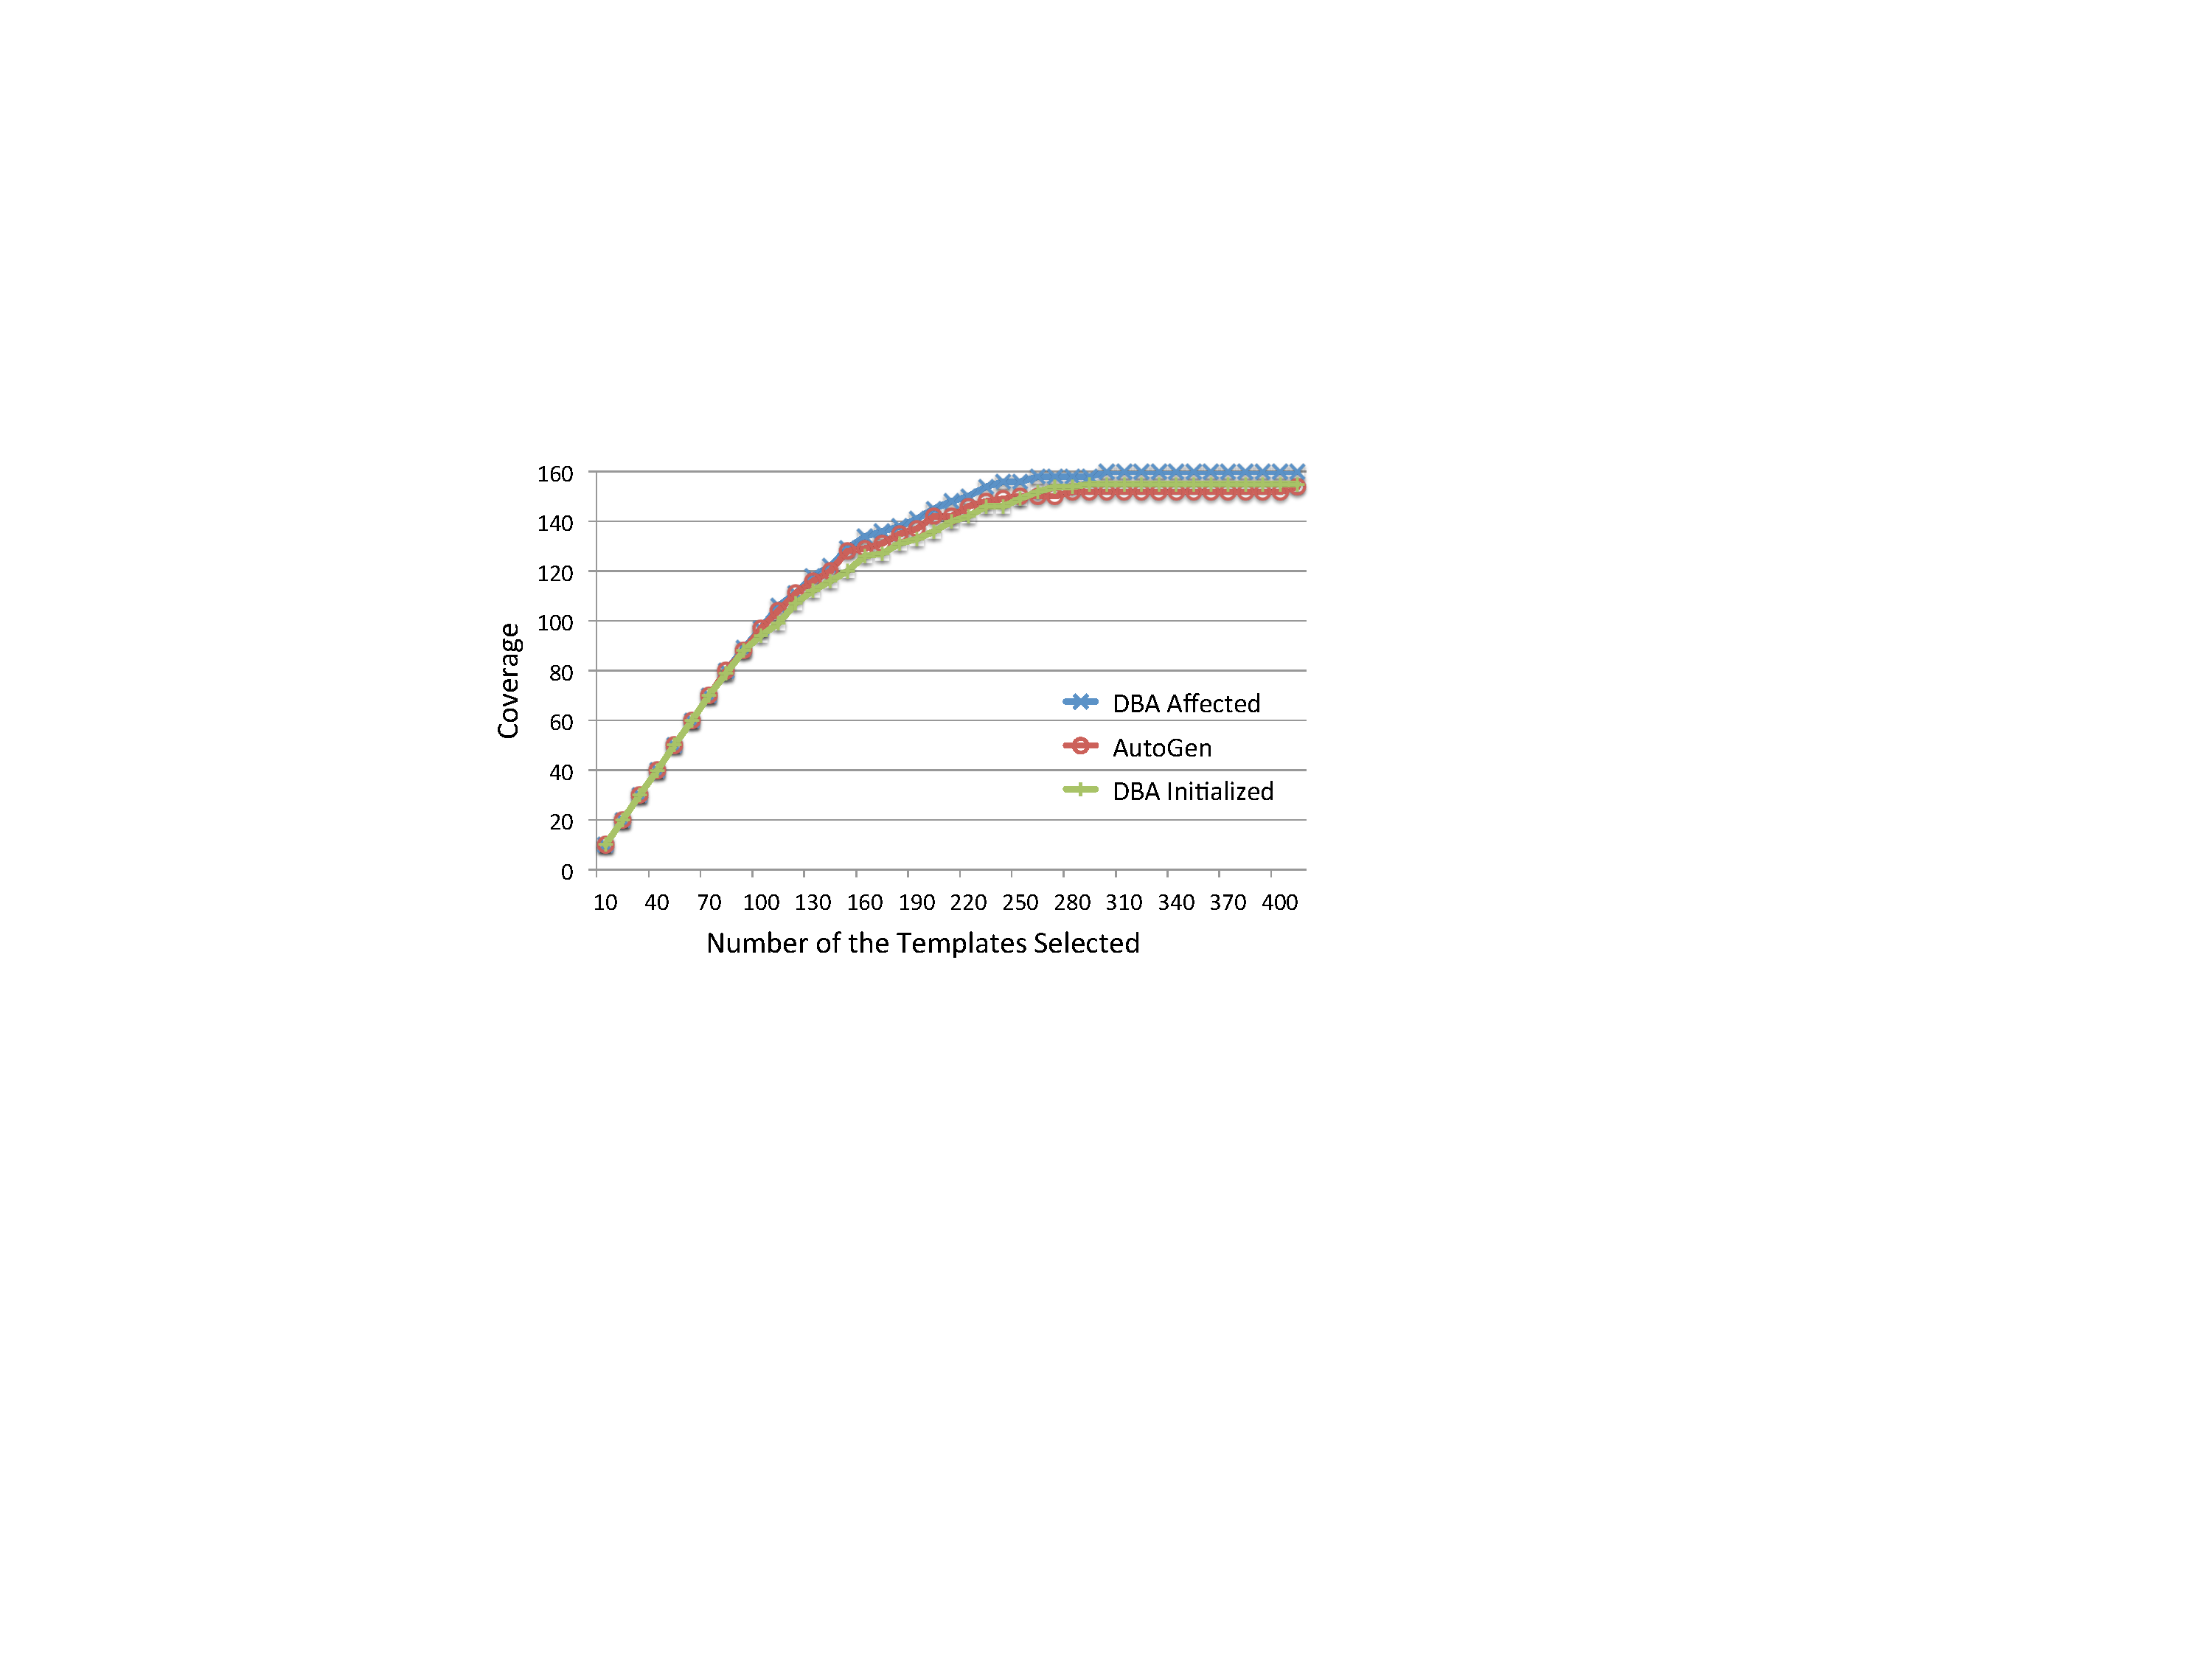
\includegraphics[width=0.9\linewidth]{pic/experimentsOffline}
  \caption{Quality of the Semantic Coverage.}
  \label{fig:experimentsOffline}
\end{figure}

\textbf{Initial Templates provided by Domain Experts.} When there is no query log available, a domain expert (such as the DBA) could specify the initial SQL templates. We note that it is difficult for a domain expert to be complete in their specification of all required templates, while it is not difficult for the expert to specify several popular templates.  Therefore, extension and smoothing is expected to make a big difference.  To evaluate this, we asked a domain expert, who often does academic searches and has a good intuition of which questions are often asked in a bibliographic database, but was not involved in the creation of $Q_{gold}$, to examine the database schema and specify the initial SQL templates. We got an initial set comprising 50 distinct SQL templates, of which 48 of were in $Q_{gold}$.  After the SQL template extension, 155 SQL templates in $Q_{gold}$ were covered in the top 1000 SQL templates. After smoothing the weights, all 155 SQL templates were ranked in the top 300 SQL templates.  Detailed results are shown in Figure~\ref{fig:experimentsOffline}.

\subsection{Online Part}
We implemented the online part of our system as a stand-alone interface that can work on top of any RDBMS.  In our current implementation, we used MySQL as the RDBMS and the Stanford Parser~\cite{Marneffe06generatingtyped} as the dependency parser.  

The online part of our system translates natural language queries into SQL statements.  The aspect we must evaluate is the precision in the translation.  We notice that this precision depends on the specific expressions used in describing the queries.  Even for describing the same query, the natural language expressions used by naive users are often different from those specified by technical users: naive users tend to use informal expressions and prefer brevity to grammatical correctness and logical precision.  So, we designed user study experiments for the online part, in which non-technical participants are recruited to specify queries in their preferred natural wording.  

\textbf{Participants.}
Sixteen Participants were recruited with flyers posted on a university campus. A questionnaire indicated that all participants were familiar with keyword search interfaces (e.g. Google), but had little knowledge of formal query languages (e.g. SQL).  Furthermore, they were fluent in both English and Chinese.  For our experiments, it is hard to convey the query task to the participants since any English description would cause bias in the task.  To overcome this, we described each query task in Chinese and asked users to compose English query sentences.  Since English and Chinese are in entirely different language families and we believe this kind of design can minimize such bias.  

\textbf{Query Task Design and Procedures.}
As mentioned in Section~\ref{subsec:experiments_offline}, the curated MAS query set $Q_{gold}$ we used in the offline part consists of the query logics that regarded by domain experts as necessary.  Moreover, $Q_{gold}$ contains various kinds of complex queries, in which 110, 52, 53, 34 queries contain aggregations, long join paths with length $\geq$ 5, subqueries, and multilevel of subqueries, respectively.  As such, we use $Q_{gold}$ to test the online part of our system.  We transform each of the query logics into a query task and evenly divide the query tasks into 16 task groups, in which each task group contains 10 query tasks.  Each participant randomly takes one task group and completes it though our system.  For each task group, the participants start with sample query tasks, in order to get familiar with each interface. 

Our system is designed to be robust. Even in the cases when the user’s input is just some keywords, for example, ``author paper most", our system is still very likely to interpret it as ``author with the most papers" rather than ``paper with the most authors", since the SQL template of the former has a higher popularity.  As such, at the beginning of each query task, users are encouraged to specify their queries in the way they like.  The initial expression for each query task is recorded for comparative experiment, since any reformulation would be affacted by the feedback of our system.

\textbf{Measurement.}
We evaluate effectiveness of the top 1 interpretation returned as $\frac{|M_P|}{|M_T|}$, in which $|M_T|$ is the total number of queries and $|M_P|$ is the number of queries that can be directly translated to the correct SQL statements.  Remember that, when ambiguity exists, our system also returns alternative interpretations for the user to choose from.  As such, we also evaluate the effectiveness of the top 5 interpretations returned as $\frac{|M_R|}{|M_T|}$, in which $M_R$ is the number of queries in which one of the candidate interpretations returned is correct.  Specifically, our system returns the user at most five candidate interpretations.  

\textbf{Comparisons.}
Our system models the natural language interpretation problem as a mapping problem, which maps the natual language query to the SQL templates in our semantic coverage.  As such, for a query task, if its corresponding SQL statement is not in the semantic coverage, the online part of our system can never handle it correctly.  As mentioned, the semantic coverage of our system is first extended and then refined based on the popularity computed generated.  Also, it can be modified by the DBAs in a semi-automatic way.  So in the comparative experiment, we test our system on five semantic coverages, which are (a) the initial semantic coverage that consists of the SQL templates directly appear in the query log, (b) the extended semantic coverage, in which additional SQL templates are generated but the weights are not smoothed, (c) the refined semantic coverage, in which the weights of SQL templates are smoothed and popular ones are selected as the semantic coverage, (d) the semantic coverage that are affected by the DBA after only two edits, and (e) the semantic coverage that is generated from the initial SQL templates provided by the DBA.  We also compare our system with NaLIR~\cite{DBLP:journals/pvldb/LiJ14}, a generic NLIDB whose semantic coverage is the syntactically valid SQL statements (under some syntactical constraints).  

\begin{figure}
  \center
  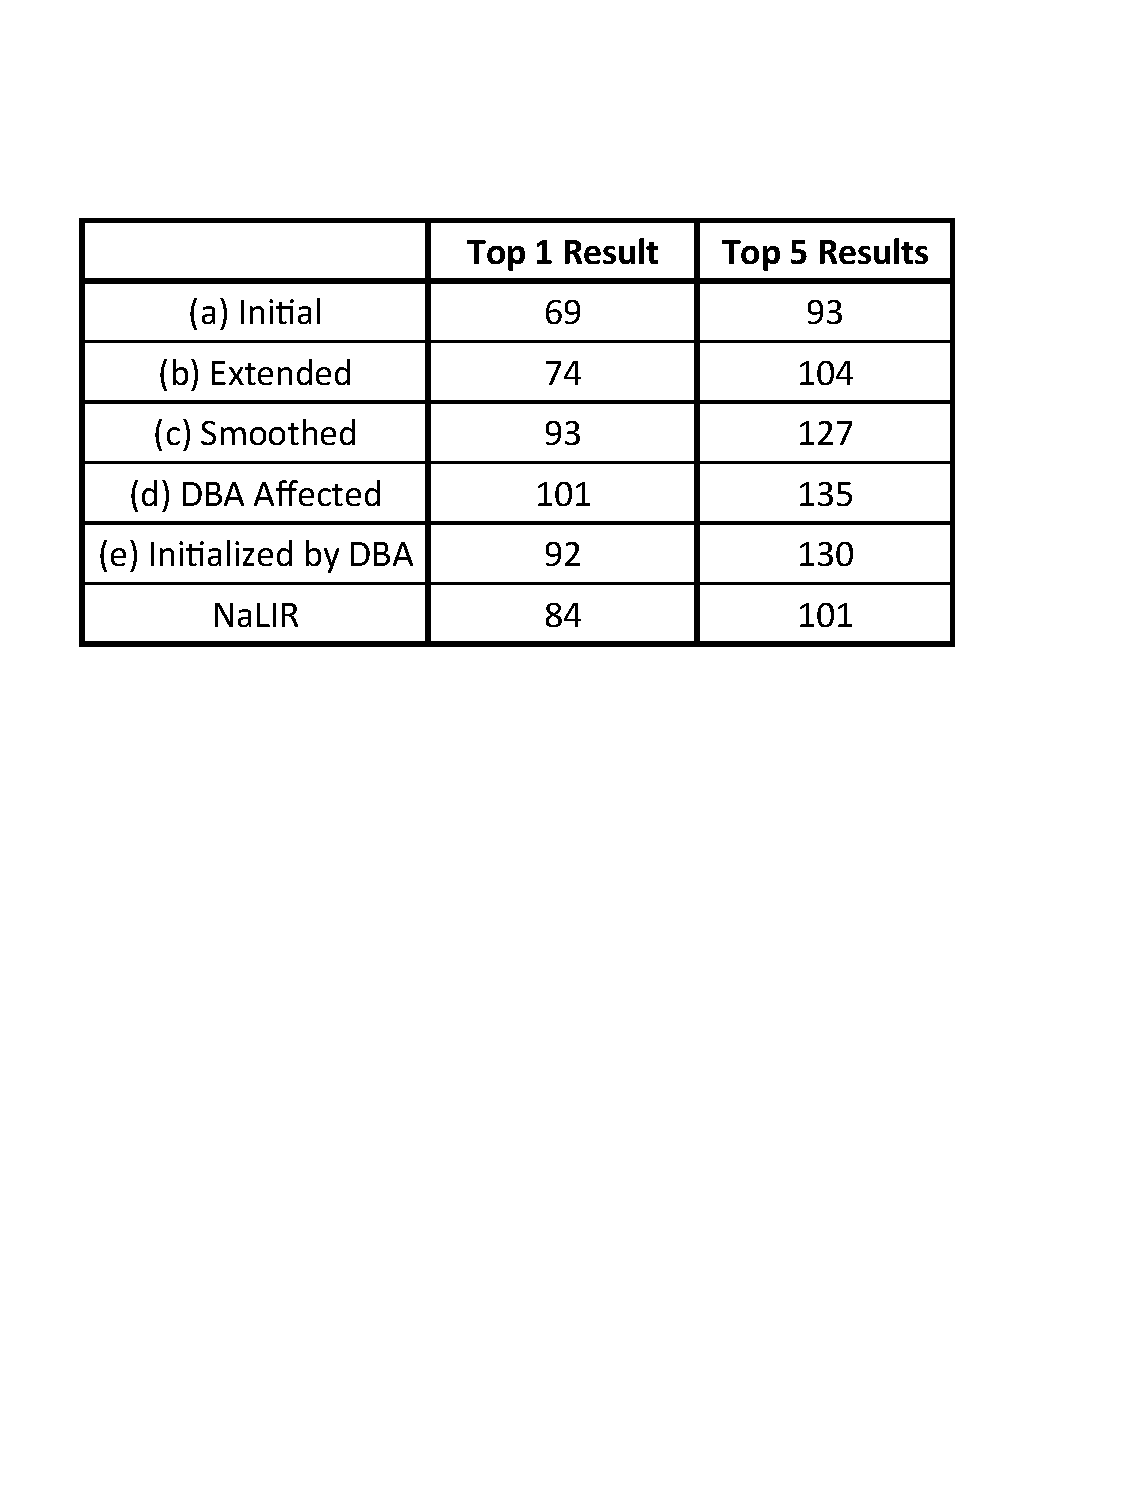
\includegraphics[width=0.75\linewidth]{pic/experimentsOnline.pdf}
  \caption{Experimental Results.}
  \label{fig:experiments}
\end{figure}

The experimental results are shown in Figure~\ref{fig:experiments}.  In experiment (a), we use query log $L$ mentioned in Section~\ref{subsec:experiments_offline} as the semantic coverage directly.  The weight of each SQL template is set as its appearing frequency with simple normalization\footnote{Add one and take the log. }.  This semantic coverage only covers 109 out of the 160 queries in the test set, which heavily limits the performance of the online part.  In experiment (b), the semantic coverage is extended from $L$, which contains 1000 SQL templates and covers 154 queries of the testing set, in which new added SQL templates are all considered as appearing once.  The performance improves but is still limited, since the unnecessary SQL templates disturb the mapping.  In experiment (c), the mapping improves a lot after the semantic coverage is refined, which contains 300 SQL templates and covers 152 queries of the testing set.   In this process, the popularity of each SQL template is computed and the SQL templates with low popularity are filtered out.  In experiment (d), as mentioned in Section~\ref{subsec:experiments_offline}, after adding two key SQL templates, the semantic coverage covers all the test queries and the performance further improves. In experiment (e), the semantic coverage is generated from the SQL templates provided by the DBA, which behaves similar to that generated from a query log.  

%=====================Related Work==========================================================
\section{Related Work}
\label{sec:relatedWork}
The problem of constructing Natural Language Interfaces to DataBases (NLIDB) has been studied for several decades.  Early systems often model the problem as a semantic parsing problem, in which grammars are either manually specified~\cite{DBLP:journals/nle/AndroutsopoulosRT95} or learned from training examples~\cite{Zelle:1996:LPD:1864519.1864543,DBLP:conf/ecml/TangM01,DBLP:bibsonomy_ge2005,DBLP:conf/acl/WongM07}.  While quite successful in some specific scenario, the grammars are hard to scale up, both to other domains and to new natural language expressions, which limits the impact~\cite{Liang:2011:LDC:2002472.2002547}.  

In recent years, deep learning methods received great success in machine translation~\cite{DBLP:journals/corr/WuSCLNMKCGMKSJL16} and question answer matching~\cite{DBLP:conf/acl/TanSXZ16,DBLP:conf/cikm/FengXZ16}.  This fact inspires researchers to apply end-to-end frameworks to build NLIDBs~\cite{DBLP:conf/acl/DongL16,DBLP:journals/debu/LuLK16,DBLP:journals/cacm/Liang16,DBLP:journals/tacl/ReddyTCKDSL16}.  From our experience, three major challenges exist in adopting end-to-end framework to construct NLIDBs.  First, the underlying database schema of different NLIDBs often differs, which means the training set used for one NLIDB cannot be applied to another.  As a result, in a real application, it is almost impossible to collect enough pairs of (NLQ, SQL) for an end-to-end model.  Second, as pointed out in~\cite{DBLP:conf/iui/PopescuEK03,DBLP:journals/pvldb/LiJ14}, reliability is very important in database applications.  Users will be very frustrated if they make wrong decisions only because they believe in the wrong results from an NLIDB.  As such, explainations are often necessary for users to understand the processing process.  However, for deep learning methods,  the intermediate structures are often unexplainable.  Third, as discussed in this paper, NLIDB has many unique resources for resolving ambiguities, like the underlying schema structure, the query log, the distribution of the data, the configuration from the DBA, and so forth.  However, in end-to-end methods, the fact that more resources taken into account often means higher dimensions of input, which would exacerbate the first problem of lacking training examples.  Consider the above obstacles, we develop a new framework instead of simply adopting their methods.  

Another branch of researches focus on building generic NLIDBs~\cite{DBLP:conf/iui/PopescuEK03,DBLP:conf/coling/PopescuAEKY04,DBLP:journals/tods/LiYJ07,DBLP:journals/pvldb/LiJ14} arose as a response to avoid the tedious configuration requirements.  PRECISE~\cite{DBLP:conf/iui/PopescuEK03,DBLP:conf/coling/PopescuAEKY04} defines a subset of natural language queries as semantically tractable queries and precisely translates these queries into corresponding SQL queries.  NaLIX~\cite{DBLP:conf/sigmod/LiYJ05} defines a domain-independent grammar for the natural language queries that are semantically expressible by XQuery and parses natural language queries to XQuery statements according to the grammar.  NaLIR~\cite{DBLP:journals/pvldb/LiJ14} is designed to support complex natural language queries, in which the semantic coverage is defined as all the syntactically valid SQL statements (with some constraints).  By transforming natural language queries to the correct points in the semantic coverage in a series steps, the queries can be translated to the desired SQL statements.  In general, existing generic NLIDBs still define their semantic coverage at the syntax level.  In our system, an offline part is used to refine the semantic coverage, which supports only the query logics that are likely to be queried.  By greatly narrowing down the semantic coverage, the burden in online mapping is reduced.  

From our point of view, the deep learning based methods and generic NLIDBs are taking two extreme strategies.  The deep learning based methods are trying to learn everything from training examples while the generic NLIDBs are avoiding training examples.  We believe that an ideal NLIDB should be provide reasonable results when cold starts and its performance can improve through the usage by collecting the user's behavior.  

Other recent works related to NLIDB would involve~\cite{DBLP:conf/sigmod/ZhengZLYSZ15,DBLP:journals/pvldb/SahaFSMMO16}. In~\cite{DBLP:conf/sigmod/ZhengZLYSZ15}, a template-based method is proposed.  In their approach, a template is defined as a natural language query template (NLT) paired with a standard query template (SQT).  Such templates are generated by joining a set of NLT and a set of SQT by measuring their similarity.   In~\cite{DBLP:journals/pvldb/SahaFSMMO16}, an intermediate ontology query language OQL serves as the target for interpreting natural language queries.  

Keyword search interfaces are widely used by non-experts to specify ad-hoc queries over relational databases~\cite{DBLP:series/synthesis/2010Yu,DBLP:conf/icde/BhalotiaHNCS02,DBLP:conf/icde/AgrawalCD02,DBLP:conf/vldb/HristidisP02}. Recently, there has been a stream of such research on keyword search~\cite{DBLP:conf/sigmod/TataL08,DBLP:journals/vldb/SimitsisKI08,DBLP:conf/sigmod/ChuBCDN09,DBLP:journals/pvldb/XinHG10,DBLP:conf/icde/FanLZ11,DBLP:journals/pvldb/BlunschiJKMS12,DBLP:journals/pvldb/BergamaschiGILV13}, in which, given a set of keywords, instead of finding the data relevant to these keywords, they try to interpret the query intent behind the keywords in the view of a formal query language. In particular, some of them extend keywords by supporting aggregation functions~\cite{DBLP:conf/sigmod/TataL08}, Boolean operators~\cite{DBLP:journals/vldb/SimitsisKI08}, query language fragments~\cite{DBLP:journals/pvldb/BlunschiJKMS12}, and so forth. These works can be considered as a first step toward addressing the challenge of natural language querying. Our work builds upon this stream of research and supports a richer query mechanism that allows us to convey much more complex semantic meaning than a flat collection of keywords.

The framework of our system is inspired from search engines~\cite{DBLP:journals/cn/BrinP98, Page99thepagerank}. Similar to NLIDBs, search engines are heuristic query systems, whose queries do not have formally defined semantic meanings. The semantic coverage of a search engine is a large set of webpages. Given a keyword query, search engines find its top mappings based on the importance of each webpage and the relevance between the keywords and each webpage.  Inspired from search engines, we model the natural language query interpretation problem as a mapping problem between the natural language query to a point in the semantic coverage.  In this framework, different kinds of resources (e.g. query log in this paper) can be naturally taken into account by affecting the mapping score in a defined mechanism.  Moreover, in this framework, some factors (e.g. importance) are pre-computed offline, while others (e.g. relevance) are computed online when a user submits a query.  We adapt this online-offline framework to NLIDBs, which helps NLIDBs to interpret natural language queries efficiently.  

A task in our system is to explain the SQL templates for the end users to choose from or for the DBA to fast review.  Previous systems explain SQL queries to users using natural language descriptions~\cite{DBLP:conf/sigmod/KokkalisVZSKI12} or query visualizations~\cite{DBLP:conf/edbt/DanaparamitaG11,DBLP:conf/icde/FanLZ11,DBLP:journals/pvldb/BergamaschiGILV13}.  In our system, we adopt the strategy used in~\cite{DBLP:conf/sigmod/KokkalisVZSKI12}.  

%=====================Conclusions==========================================================
\section{Conclusion and Future Work}
\label{sec:conclusion}

In this paper, we provide a framework for constructing natural language query interfaces over relational databases.  In the framework, the semantic coverage of an NLIDB is defined as a set of weighted SQL templates, in which the weight describes the likelihood of a SQL template to be queried.  Given a natural language query, by mapping it to the correct SQL template in the semantic coverage, the query can be translated into the desired SQL statement, which may include comparison predicates, conjunctions, quantifications, multi-level aggregations, nestings, and various types of joins, among other things.  We provide the principled strategy for automatically generating the semantic coverage from the query log.  Also, an effective mapping strategy, which considers the template weights, as well as the relevance between the query and the templates, is proposed.  The framework described in this paper has been implemented, and actual user experience gathered.  Using our system, a small sized query log is enough to generate the necessary SQL templates, and even naive users are able to accomplish logically complex query tasks against our system.   

In our current implementation, the online part is major based on the similarity metric between the natural language and the SQL templates.  In the future, training examples like pairs of NLQ and SQL will be considered.  We would like to merge the metric-based methods with learning-based methods.  We hope that the system can provide reasonable results in the cases when there is no training examples and its performance would improve when training examples are gathered through the usage.    

\bibliographystyle{abbrv}
\bibliography{my-bib-database}
\end{document} 